\documentclass[1p]{elsarticle_modified}
%\bibliographystyle{elsarticle-num}

%\usepackage[colorlinks]{hyperref}
%\usepackage{abbrmath_seonhwa} %\Abb, \Ascr, \Acal ,\Abf, \Afrak
\usepackage{amsfonts}
\usepackage{amssymb}
\usepackage{amsmath}
\usepackage{amsthm}
\usepackage{scalefnt}
\usepackage{amsbsy}
\usepackage{kotex}
\usepackage{caption}
\usepackage{subfig}
\usepackage{color}
\usepackage{graphicx}
\usepackage{xcolor} %% white, black, red, green, blue, cyan, magenta, yellow
\usepackage{float}
\usepackage{setspace}
\usepackage{hyperref}

\usepackage{tikz}
\usetikzlibrary{arrows}

\usepackage{multirow}
\usepackage{array} % fixed length table
\usepackage{hhline}

%%%%%%%%%%%%%%%%%%%%%
\makeatletter
\renewcommand*\env@matrix[1][\arraystretch]{%
	\edef\arraystretch{#1}%
	\hskip -\arraycolsep
	\let\@ifnextchar\new@ifnextchar
	\array{*\c@MaxMatrixCols c}}
\makeatother %https://tex.stackexchange.com/questions/14071/how-can-i-increase-the-line-spacing-in-a-matrix
%%%%%%%%%%%%%%%

\usepackage[normalem]{ulem}

\newcommand{\msout}[1]{\ifmmode\text{\sout{\ensuremath{#1}}}\else\sout{#1}\fi}
%SOURCE: \msout is \stkout macro in https://tex.stackexchange.com/questions/20609/strikeout-in-math-mode

\newcommand{\cancel}[1]{
	\ifmmode
	{\color{red}\msout{#1}}
	\else
	{\color{red}\sout{#1}}
	\fi
}

\newcommand{\add}[1]{
	{\color{blue}\uwave{#1}}
}

\newcommand{\replace}[2]{
	\ifmmode
	{\color{red}\msout{#1}}{\color{blue}\uwave{#2}}
	\else
	{\color{red}\sout{#1}}{\color{blue}\uwave{#2}}
	\fi
}

\newcommand{\Sol}{\mathcal{S}} %segment
\newcommand{\D}{D} %diagram
\newcommand{\A}{\mathcal{A}} %arc


%%%%%%%%%%%%%%%%%%%%%%%%%%%%%5 test

\def\sl{\operatorname{\textup{SL}}(2,\Cbb)}
\def\psl{\operatorname{\textup{PSL}}(2,\Cbb)}
\def\quan{\mkern 1mu \triangleright \mkern 1mu}

\theoremstyle{definition}
\newtheorem{thm}{Theorem}[section]
\newtheorem{prop}[thm]{Proposition}
\newtheorem{lem}[thm]{Lemma}
\newtheorem{ques}[thm]{Question}
\newtheorem{cor}[thm]{Corollary}
\newtheorem{defn}[thm]{Definition}
\newtheorem{exam}[thm]{Example}
\newtheorem{rmk}[thm]{Remark}
\newtheorem{alg}[thm]{Algorithm}

\newcommand{\I}{\sqrt{-1}}
\begin{document}

%\begin{frontmatter}
%
%\title{Boundary parabolic representations of knots up to 8 crossings}
%
%%% Group authors per affiliation:
%\author{Yunhi Cho} 
%\address{Department of Mathematics, University of Seoul, Seoul, Korea}
%\ead{yhcho@uos.ac.kr}
%
%
%\author{Seonhwa Kim} %\fnref{s_kim}}
%\address{Center for Geometry and Physics, Institute for Basic Science, Pohang, 37673, Korea}
%\ead{ryeona17@ibs.re.kr}
%
%\author{Hyuk Kim}
%\address{Department of Mathematical Sciences, Seoul National University, Seoul 08826, Korea}
%\ead{hyukkim@snu.ac.kr}
%
%\author{Seokbeom Yoon}
%\address{Department of Mathematical Sciences, Seoul National University, Seoul, 08826,  Korea}
%\ead{sbyoon15@snu.ac.kr}
%
%\begin{abstract}
%We find all boundary parabolic representation of knots up to 8 crossings.
%
%\end{abstract}
%\begin{keyword}
%    \MSC[2010] 57M25 
%\end{keyword}
%
%\end{frontmatter}

%\linenumbers
%\tableofcontents
%
\newcommand\colored[1]{\textcolor{white}{\rule[-0.35ex]{0.8em}{1.4ex}}\kern-0.8em\color{red} #1}%
%\newcommand\colored[1]{\textcolor{white}{ #1}\kern-2.17ex	\textcolor{white}{ #1}\kern-1.81ex	\textcolor{white}{ #1}\kern-2.15ex\color{red}#1	}

{\Large $\underline{12a_{0167}~(K12a_{0167})}$}

\setlength{\tabcolsep}{10pt}
\renewcommand{\arraystretch}{1.6}
\vspace{1cm}\begin{tabular}{m{100pt}>{\centering\arraybackslash}m{274pt}}
\multirow{5}{120pt}{
	\centering
	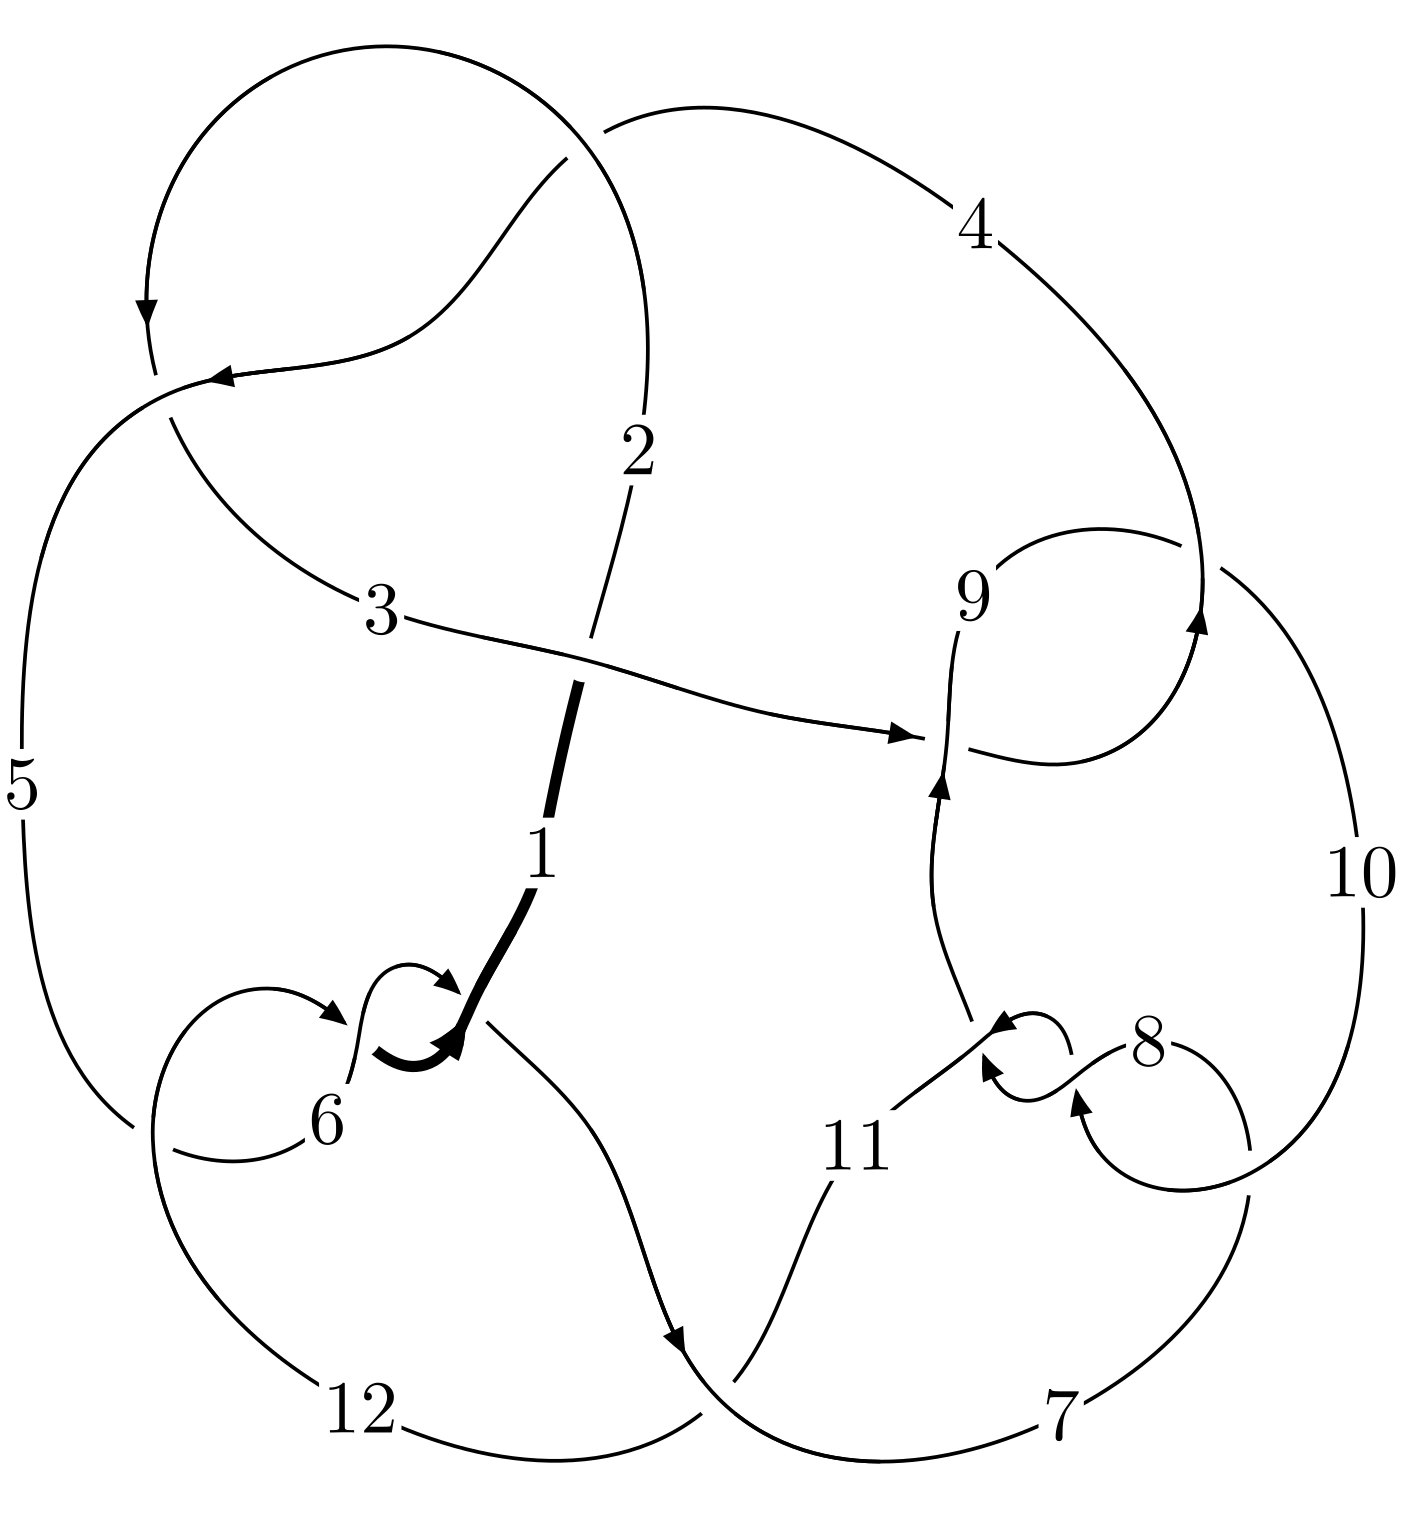
\includegraphics[width=112pt]{../../../GIT/diagram.site/Diagrams/png/968_12a_0167.png}\\
\ \ \ A knot diagram\footnotemark}&
\allowdisplaybreaks
\textbf{Linearized knot diagam} \\
\cline{2-2}
 &
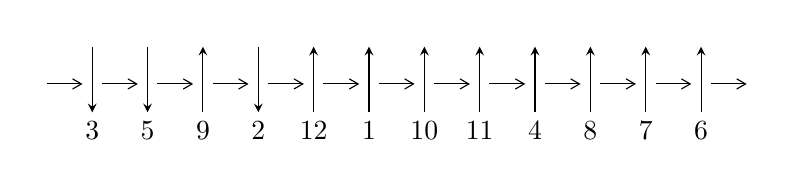
\begin{tikzpicture}[x=20pt, y=17pt]
	% nodes
	\node (C0) at (0, 0) {};
	\node (C1) at (1, 0) {};
	\node (C1U) at (1, +1) {};
	\node (C1D) at (1, -1) {3};

	\node (C2) at (2, 0) {};
	\node (C2U) at (2, +1) {};
	\node (C2D) at (2, -1) {5};

	\node (C3) at (3, 0) {};
	\node (C3U) at (3, +1) {};
	\node (C3D) at (3, -1) {9};

	\node (C4) at (4, 0) {};
	\node (C4U) at (4, +1) {};
	\node (C4D) at (4, -1) {2};

	\node (C5) at (5, 0) {};
	\node (C5U) at (5, +1) {};
	\node (C5D) at (5, -1) {12};

	\node (C6) at (6, 0) {};
	\node (C6U) at (6, +1) {};
	\node (C6D) at (6, -1) {1};

	\node (C7) at (7, 0) {};
	\node (C7U) at (7, +1) {};
	\node (C7D) at (7, -1) {10};

	\node (C8) at (8, 0) {};
	\node (C8U) at (8, +1) {};
	\node (C8D) at (8, -1) {11};

	\node (C9) at (9, 0) {};
	\node (C9U) at (9, +1) {};
	\node (C9D) at (9, -1) {4};

	\node (C10) at (10, 0) {};
	\node (C10U) at (10, +1) {};
	\node (C10D) at (10, -1) {8};

	\node (C11) at (11, 0) {};
	\node (C11U) at (11, +1) {};
	\node (C11D) at (11, -1) {7};

	\node (C12) at (12, 0) {};
	\node (C12U) at (12, +1) {};
	\node (C12D) at (12, -1) {6};
	\node (C13) at (13, 0) {};

	% arrows
	\draw[->,>={angle 60}]
	(C0) edge (C1) (C1) edge (C2) (C2) edge (C3) (C3) edge (C4) (C4) edge (C5) (C5) edge (C6) (C6) edge (C7) (C7) edge (C8) (C8) edge (C9) (C9) edge (C10) (C10) edge (C11) (C11) edge (C12) (C12) edge (C13) ;	\draw[->,>=stealth]
	(C1U) edge (C1D) (C2U) edge (C2D) (C3D) edge (C3U) (C4U) edge (C4D) (C5D) edge (C5U) (C6D) edge (C6U) (C7D) edge (C7U) (C8D) edge (C8U) (C9D) edge (C9U) (C10D) edge (C10U) (C11D) edge (C11U) (C12D) edge (C12U) ;
	\end{tikzpicture} \\
\hhline{~~} \\& 
\textbf{Solving Sequence} \\ \cline{2-2} 
 &
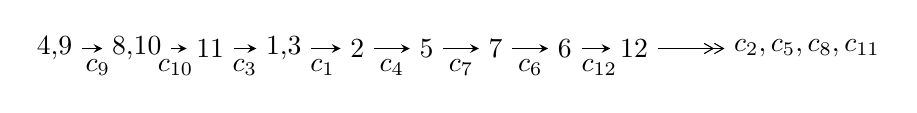
\begin{tikzpicture}[x=25pt, y=7pt]
	% node
	\node (A0) at (-1/8, 0) {4,9};
	\node (A1) at (17/16, 0) {8,10};
	\node (A2) at (17/8, 0) {11};
	\node (A3) at (51/16, 0) {1,3};
	\node (A4) at (17/4, 0) {2};
	\node (A5) at (21/4, 0) {5};
	\node (A6) at (25/4, 0) {7};
	\node (A7) at (29/4, 0) {6};
	\node (A8) at (33/4, 0) {12};
	\node (C1) at (1/2, -1) {$c_{9}$};
	\node (C2) at (13/8, -1) {$c_{10}$};
	\node (C3) at (21/8, -1) {$c_{3}$};
	\node (C4) at (15/4, -1) {$c_{1}$};
	\node (C5) at (19/4, -1) {$c_{4}$};
	\node (C6) at (23/4, -1) {$c_{7}$};
	\node (C7) at (27/4, -1) {$c_{6}$};
	\node (C8) at (31/4, -1) {$c_{12}$};
	\node (A9) at (43/4, 0) {$c_{2},c_{5},c_{8},c_{11}$};

	% edge
	\draw[->,>=stealth]	
	(A0) edge (A1) (A1) edge (A2) (A2) edge (A3) (A3) edge (A4) (A4) edge (A5) (A5) edge (A6) (A6) edge (A7) (A7) edge (A8) ;
	\draw[->>,>={angle 60}]	
	(A8) edge (A9);
\end{tikzpicture} \\ 

\end{tabular} \\

\footnotetext{
The image of knot diagram is generated by the software ``\textbf{Draw programme}" developed by Andrew Bartholomew(\url{http://www.layer8.co.uk/maths/draw/index.htm\#Running-draw}), where we modified some parts for our purpose(\url{https://github.com/CATsTAILs/LinksPainter}).
}\phantom \\ \newline 
\centering \textbf{Ideals for irreducible components\footnotemark of $X_{\text{par}}$} 
 
\begin{align*}
I^u_{1}&=\langle 
-179878036 u^{22}-223200067 u^{21}+\cdots+15409974654 d-115530422,\\
\phantom{I^u_{1}}&\phantom{= \langle  }487430093 u^{22}+2626639316 u^{21}+\cdots+184919695848 c-182635192736,\\
\phantom{I^u_{1}}&\phantom{= \langle  }6729099212 u^{22}+11896606493 u^{21}+\cdots+92459847924 b+39193550776,\\
\phantom{I^u_{1}}&\phantom{= \langle  }-321494617 u^{22}+1287799250 u^{21}+\cdots+92459847924 a-91427201564,\\
\phantom{I^u_{1}}&\phantom{= \langle  }u^{23}+2 u^{22}+\cdots-4 u^2+8\rangle \\
I^u_{2}&=\langle 
u^2 c- u^3- c u+u^2+d+c-1,\;-2 u^3 c+3 u^2 c+u^3+c^2-2 c u- u^2+u,\;u^2+b+1,\;u^3-2 u^2+a+u-1,\\
\phantom{I^u_{2}}&\phantom{= \langle  }u^4-2 u^3+2 u^2- u+1\rangle \\
I^u_{3}&=\langle 
- u^7+u^5-2 u^3+d+u,\;u^5+c+u,\;- u^7- u^6+u^4- a u+b+1,\\
\phantom{I^u_{3}}&\phantom{= \langle  }- u^7 a+u^7+2 u^5 a+2 u^4 a-2 u^5-2 u^3 a- u^4-2 u^2 a+3 u^3+a^2+u^2+2 a-2,\\
\phantom{I^u_{3}}&\phantom{= \langle  }u^8+u^7- u^6-2 u^5+u^4+2 u^3-2 u-1\rangle \\
I^u_{4}&=\langle 
- u^6- u^5+u^4- u^2 a+2 u^3- a u+d- u-1,\\
\phantom{I^u_{4}}&\phantom{= \langle  }2 u^7 a+2 u^6 a- u^7-2 u^5 a- u^6-4 u^4 a+u^5+2 u^3 a+3 u^4+3 u^2 a- a u-2 u^2+c-3 a- u+1,\\
\phantom{I^u_{4}}&\phantom{= \langle  }- u^7- u^6+u^4- a u+b+1,\;- u^7 a+u^7+2 u^5 a+2 u^4 a-2 u^5-2 u^3 a- u^4-2 u^2 a+3 u^3+a^2+u^2+2 a-2,\\
\phantom{I^u_{4}}&\phantom{= \langle  }u^8+u^7- u^6-2 u^5+u^4+2 u^3-2 u-1\rangle \\
I^u_{5}&=\langle 
- u^7+u^5-2 u^3+d+u,\;u^5+c+u,\;- u^7- u^6+2 u^5+3 u^4-2 u^3-4 u^2+b+2 u+3,\\
\phantom{I^u_{5}}&\phantom{= \langle  }u^7-2 u^5-2 u^4+2 u^3+2 u^2+a-2 u-2,\;u^8+u^7- u^6-2 u^5+u^4+2 u^3-2 u-1\rangle \\
I^u_{6}&=\langle 
u^5 c- u^4 c-2 u^3 c+3 u^2 c+u^3+c u+d-2 c- u,\\
\phantom{I^u_{6}}&\phantom{= \langle  }-3 u^5 c- u^4 c+u^5+5 u^3 c+u^4-3 u^2 c-3 u^3+2 c^2-5 c u+u^2+6 c+3 u-4,\;- u^4+u^2+b- u-1,\\
\phantom{I^u_{6}}&\phantom{= \langle  }- u^5+u^4+3 u^3-3 u^2+2 a- u+4,\;u^6- u^5- u^4+3 u^3- u^2-2 u+2\rangle \\
\\
I^v_{1}&=\langle 
c,\;d-1,\;b,\;a+1,\;v+1\rangle \\
I^v_{2}&=\langle 
a,\;d,\;c-1,\;b+1,\;v-1\rangle \\
I^v_{3}&=\langle 
a,\;d-1,\;c+a-1,\;b+1,\;v-1\rangle \\
I^v_{4}&=\langle 
c,\;d-1,\;a v+c+v-1,\;b v+1\rangle \\
\end{align*}
\raggedright * 9 irreducible components of $\dim_{\mathbb{C}}=0$, with total 86 representations.\\
\raggedright * 1 irreducible components of $\dim_{\mathbb{C}}=1$ \\
\footnotetext{All coefficients of polynomials are rational numbers. But the coefficients are sometimes approximated in decimal forms when there is not enough margin.}
\newpage
\renewcommand{\arraystretch}{1}
\centering \section*{I. $I^u_{1}= \langle -1.80\times10^{8} u^{22}-2.23\times10^{8} u^{21}+\cdots+1.54\times10^{10} d-1.16\times10^{8},\;4.87\times10^{8} u^{22}+2.63\times10^{9} u^{21}+\cdots+1.85\times10^{11} c-1.83\times10^{11},\;6.73\times10^{9} u^{22}+1.19\times10^{10} u^{21}+\cdots+9.25\times10^{10} b+3.92\times10^{10},\;-3.21\times10^{8} u^{22}+1.29\times10^{9} u^{21}+\cdots+9.25\times10^{10} a-9.14\times10^{10},\;u^{23}+2 u^{22}+\cdots-4 u^2+8 \rangle$}
\flushleft \textbf{(i) Arc colorings}\\
\begin{tabular}{m{7pt} m{180pt} m{7pt} m{180pt} }
\flushright $a_{4}=$&$\begin{pmatrix}0\\u\end{pmatrix}$ \\
\flushright $a_{9}=$&$\begin{pmatrix}1\\0\end{pmatrix}$ \\
\flushright $a_{8}=$&$\begin{pmatrix}-0.00263590 u^{22}-0.0142042 u^{21}+\cdots-0.0222392 u+0.987646\\0.0116728 u^{22}+0.0144841 u^{21}+\cdots-0.162782 u+0.00749712\end{pmatrix}$ \\
\flushright $a_{10}=$&$\begin{pmatrix}1\\- u^2\end{pmatrix}$ \\
\flushright $a_{11}=$&$\begin{pmatrix}-0.00263590 u^{22}-0.0142042 u^{21}+\cdots-0.0222392 u+0.987646\\-0.0165392 u^{22}-0.0250589 u^{21}+\cdots+0.141695 u-0.0789564\end{pmatrix}$ \\
\flushright $a_{1}=$&$\begin{pmatrix}0.00347713 u^{22}-0.0139282 u^{21}+\cdots-0.640963 u+0.988831\\-0.0727786 u^{22}-0.128668 u^{21}+\cdots+0.850224 u-0.423898\end{pmatrix}$ \\
\flushright $a_{3}=$&$\begin{pmatrix}- u\\u\end{pmatrix}$ \\
\flushright $a_{2}=$&$\begin{pmatrix}0.0160451 u^{22}-0.0132319 u^{21}+\cdots-1.19538 u+0.956887\\-0.0853466 u^{22}-0.129364 u^{21}+\cdots+1.40464 u-0.391954\end{pmatrix}$ \\
\flushright $a_{5}=$&$\begin{pmatrix}0.0693015 u^{22}+0.142596 u^{21}+\cdots-0.209260 u-0.564933\\-0.0853466 u^{22}-0.129364 u^{21}+\cdots+1.40464 u-0.391954\end{pmatrix}$ \\
\flushright $a_{7}=$&$\begin{pmatrix}-0.0191751 u^{22}-0.0392631 u^{21}+\cdots+0.119456 u+0.908690\\0.0174433 u^{22}+0.0237607 u^{21}+\cdots-0.295096 u+0.0716533\end{pmatrix}$ \\
\flushright $a_{6}=$&$\begin{pmatrix}-0.0462554 u^{22}-0.0937250 u^{21}+\cdots+0.159204 u+0.719639\\0.0587694 u^{22}+0.0800767 u^{21}+\cdots-0.985189 u+0.264336\end{pmatrix}$ \\
\flushright $a_{12}=$&$\begin{pmatrix}-0.00173177 u^{22}-0.0155024 u^{21}+\cdots-0.175640 u+0.980343\\-0.0358544 u^{22}-0.0587621 u^{21}+\cdots+0.281242 u-0.167964\end{pmatrix}$\\&\end{tabular}
\flushleft \textbf{(ii) Obstruction class $= -1$}\\~\\
\flushleft \textbf{(iii) Cusp Shapes $= \frac{15567855023}{46229923962} u^{22}+\frac{8703838979}{46229923962} u^{21}+\cdots-\frac{168604101146}{23114961981} u+\frac{87470148380}{23114961981}$}\\~\\
\newpage\renewcommand{\arraystretch}{1}
\flushleft \textbf{(iv) u-Polynomials at the component}\newline \\
\begin{tabular}{m{50pt}|m{274pt}}
Crossings & \hspace{64pt}u-Polynomials at each crossing \\
\hline $$\begin{aligned}c_{1}\end{aligned}$$&$\begin{aligned}
&u^{23}+10 u^{22}+\cdots+88 u+16
\end{aligned}$\\
\hline $$\begin{aligned}c_{2},c_{4}\end{aligned}$$&$\begin{aligned}
&u^{23}-2 u^{22}+\cdots+8 u-4
\end{aligned}$\\
\hline $$\begin{aligned}c_{3},c_{9}\end{aligned}$$&$\begin{aligned}
&u^{23}-2 u^{22}+\cdots+4 u^2-8
\end{aligned}$\\
\hline $$\begin{aligned}c_{5},c_{6},c_{7}\\c_{8},c_{10},c_{12}\end{aligned}$$&$\begin{aligned}
&u^{23}+2 u^{22}+\cdots- u-1
\end{aligned}$\\
\hline $$\begin{aligned}c_{11}\end{aligned}$$&$\begin{aligned}
&u^{23}-6 u^{22}+\cdots+64 u-64
\end{aligned}$\\
\hline
\end{tabular}\\~\\
\newpage\renewcommand{\arraystretch}{1}
\flushleft \textbf{(v) Riley Polynomials at the component}\newline \\
\begin{tabular}{m{50pt}|m{274pt}}
Crossings & \hspace{64pt}Riley Polynomials at each crossing \\
\hline $$\begin{aligned}c_{1}\end{aligned}$$&$\begin{aligned}
&y^{23}+6 y^{22}+\cdots+1824 y-256
\end{aligned}$\\
\hline $$\begin{aligned}c_{2},c_{4}\end{aligned}$$&$\begin{aligned}
&y^{23}-10 y^{22}+\cdots+88 y-16
\end{aligned}$\\
\hline $$\begin{aligned}c_{3},c_{9}\end{aligned}$$&$\begin{aligned}
&y^{23}-6 y^{22}+\cdots+64 y-64
\end{aligned}$\\
\hline $$\begin{aligned}c_{5},c_{6},c_{7}\\c_{8},c_{10},c_{12}\end{aligned}$$&$\begin{aligned}
&y^{23}-24 y^{22}+\cdots-9 y-1
\end{aligned}$\\
\hline $$\begin{aligned}c_{11}\end{aligned}$$&$\begin{aligned}
&y^{23}+10 y^{22}+\cdots-6144 y-4096
\end{aligned}$\\
\hline
\end{tabular}\\~\\
\newpage\flushleft \textbf{(vi) Complex Volumes and Cusp Shapes}
$$\begin{array}{c|c|c}  
\text{Solutions to }I^u_{1}& \I (\text{vol} + \sqrt{-1}CS) & \text{Cusp shape}\\
 \hline 
\begin{aligned}
u &= -0.758227 + 0.807207 I \\
a &= -1.18253 + 1.19256 I \\
b &= -0.21429 - 1.43213 I \\
c &= \phantom{-}0.632217 + 0.500472 I \\
d &= -0.591761 + 0.042510 I\end{aligned}
 & -5.90461 + 1.36538 I & -0.279938 - 0.826772 I \\ \hline\begin{aligned}
u &= -0.758227 - 0.807207 I \\
a &= -1.18253 - 1.19256 I \\
b &= -0.21429 + 1.43213 I \\
c &= \phantom{-}0.632217 - 0.500472 I \\
d &= -0.591761 - 0.042510 I\end{aligned}
 & -5.90461 - 1.36538 I & -0.279938 + 0.826772 I \\ \hline\begin{aligned}
u &= \phantom{-}0.830705 + 0.204801 I \\
a &= -0.258089 + 0.246069 I \\
b &= \phantom{-}0.666656 - 1.123170 I \\
c &= \phantom{-}0.629069 - 0.215069 I \\
d &= -0.057606 + 0.411947 I\end{aligned}
 & \phantom{-}0.25505 + 3.01929 I & \phantom{-}7.24264 - 9.08374 I \\ \hline\begin{aligned}
u &= \phantom{-}0.830705 - 0.204801 I \\
a &= -0.258089 - 0.246069 I \\
b &= \phantom{-}0.666656 + 1.123170 I \\
c &= \phantom{-}0.629069 + 0.215069 I \\
d &= -0.057606 - 0.411947 I\end{aligned}
 & \phantom{-}0.25505 - 3.01929 I & \phantom{-}7.24264 + 9.08374 I \\ \hline\begin{aligned}
u &= \phantom{-}0.112218 + 1.144740 I \\
a &= -0.511153 - 0.296391 I \\
b &= \phantom{-}1.40432 + 0.22505 I \\
c &= \phantom{-}0.417690 + 0.009308 I \\
d &= \phantom{-}1.93741 - 0.14856 I\end{aligned}
 & \phantom{-}8.23677 - 2.50119 I & \phantom{-}13.28602 + 3.12140 I \\ \hline\begin{aligned}
u &= \phantom{-}0.112218 - 1.144740 I \\
a &= -0.511153 + 0.296391 I \\
b &= \phantom{-}1.40432 - 0.22505 I \\
c &= \phantom{-}0.417690 - 0.009308 I \\
d &= \phantom{-}1.93741 + 0.14856 I\end{aligned}
 & \phantom{-}8.23677 + 2.50119 I & \phantom{-}13.28602 - 3.12140 I\\
 \hline 
 \end{array}$$\newpage$$\begin{array}{c|c|c}  
\text{Solutions to }I^u_{1}& \I (\text{vol} + \sqrt{-1}CS) & \text{Cusp shape}\\
 \hline 
\begin{aligned}
u &= \phantom{-}0.561270 + 1.026650 I \\
a &= -0.390779 - 1.343850 I \\
b &= -0.15516 + 1.60423 I \\
c &= \phantom{-}0.423044 + 0.049165 I \\
d &= \phantom{-}1.70161 - 0.72226 I\end{aligned}
 & \phantom{-}5.56899 - 4.43236 I & \phantom{-}12.33564 + 2.61344 I \\ \hline\begin{aligned}
u &= \phantom{-}0.561270 - 1.026650 I \\
a &= -0.390779 + 1.343850 I \\
b &= -0.15516 - 1.60423 I \\
c &= \phantom{-}0.423044 - 0.049165 I \\
d &= \phantom{-}1.70161 + 0.72226 I\end{aligned}
 & \phantom{-}5.56899 + 4.43236 I & \phantom{-}12.33564 - 2.61344 I \\ \hline\begin{aligned}
u &= -0.972761 + 0.735330 I \\
a &= -1.43485 + 0.61545 I \\
b &= \phantom{-}1.26169 - 1.93679 I \\
c &= \phantom{-}0.564139 + 0.426386 I \\
d &= -0.710629 - 0.218537 I\end{aligned}
 & -5.23569 - 7.16228 I & \phantom{-}1.72036 + 6.58026 I \\ \hline\begin{aligned}
u &= -0.972761 - 0.735330 I \\
a &= -1.43485 - 0.61545 I \\
b &= \phantom{-}1.26169 + 1.93679 I \\
c &= \phantom{-}0.564139 - 0.426386 I \\
d &= -0.710629 + 0.218537 I\end{aligned}
 & -5.23569 + 7.16228 I & \phantom{-}1.72036 - 6.58026 I \\ \hline\begin{aligned}
u &= -0.701924 + 1.071670 I \\
a &= -0.21749 + 1.49119 I \\
b &= -1.06220 - 1.62478 I \\
c &= \phantom{-}0.415821 - 0.060496 I \\
d &= \phantom{-}1.71873 + 0.92854 I\end{aligned}
 & \phantom{-}2.90411 + 9.45510 I & \phantom{-}9.09507 - 6.28090 I \\ \hline\begin{aligned}
u &= -0.701924 - 1.071670 I \\
a &= -0.21749 - 1.49119 I \\
b &= -1.06220 + 1.62478 I \\
c &= \phantom{-}0.415821 + 0.060496 I \\
d &= \phantom{-}1.71873 - 0.92854 I\end{aligned}
 & \phantom{-}2.90411 - 9.45510 I & \phantom{-}9.09507 + 6.28090 I\\
 \hline 
 \end{array}$$\newpage$$\begin{array}{c|c|c}  
\text{Solutions to }I^u_{1}& \I (\text{vol} + \sqrt{-1}CS) & \text{Cusp shape}\\
 \hline 
\begin{aligned}
u &= -1.324650 + 0.201985 I \\
a &= \phantom{-}1.23370 + 0.73880 I \\
b &= -1.082960 + 0.067487 I \\
c &= -2.00719 - 0.40410 I \\
d &= \phantom{-}2.17756 - 0.28510 I\end{aligned}
 & \phantom{-}13.75320 - 2.16453 I & \phantom{-}16.4022 + 0.8027 I \\ \hline\begin{aligned}
u &= -1.324650 - 0.201985 I \\
a &= \phantom{-}1.23370 - 0.73880 I \\
b &= -1.082960 - 0.067487 I \\
c &= -2.00719 + 0.40410 I \\
d &= \phantom{-}2.17756 + 0.28510 I\end{aligned}
 & \phantom{-}13.75320 + 2.16453 I & \phantom{-}16.4022 - 0.8027 I \\ \hline\begin{aligned}
u &= \phantom{-}1.140080 + 0.732610 I \\
a &= -1.76969 - 0.67662 I \\
b &= \phantom{-}1.39872 + 1.26269 I \\
c &= -1.39259 + 1.27651 I \\
d &= \phantom{-}1.80476 + 0.99453 I\end{aligned}
 & \phantom{-}7.42067 + 10.78250 I & \phantom{-}12.9034 - 6.4003 I \\ \hline\begin{aligned}
u &= \phantom{-}1.140080 - 0.732610 I \\
a &= -1.76969 + 0.67662 I \\
b &= \phantom{-}1.39872 - 1.26269 I \\
c &= -1.39259 - 1.27651 I \\
d &= \phantom{-}1.80476 - 0.99453 I\end{aligned}
 & \phantom{-}7.42067 - 10.78250 I & \phantom{-}12.9034 + 6.4003 I \\ \hline\begin{aligned}
u &= \phantom{-}1.315590 + 0.366431 I \\
a &= \phantom{-}0.530331 - 1.007860 I \\
b &= -0.511464 - 0.076354 I \\
c &= -1.85311 + 0.68498 I \\
d &= \phantom{-}2.14413 + 0.51761 I\end{aligned}
 & \phantom{-}12.6616 + 7.9478 I & \phantom{-}14.6243 - 6.1519 I \\ \hline\begin{aligned}
u &= \phantom{-}1.315590 - 0.366431 I \\
a &= \phantom{-}0.530331 + 1.007860 I \\
b &= -0.511464 + 0.076354 I \\
c &= -1.85311 - 0.68498 I \\
d &= \phantom{-}2.14413 - 0.51761 I\end{aligned}
 & \phantom{-}12.6616 - 7.9478 I & \phantom{-}14.6243 + 6.1519 I\\
 \hline 
 \end{array}$$\newpage$$\begin{array}{c|c|c}  
\text{Solutions to }I^u_{1}& \I (\text{vol} + \sqrt{-1}CS) & \text{Cusp shape}\\
 \hline 
\begin{aligned}
u &= -0.618010\phantom{ +0.000000I} \\
a &= \phantom{-}0.764150\phantom{ +0.000000I} \\
b &= -1.38261\phantom{ +0.000000I} \\
c &= \phantom{-}0.651263\phantom{ +0.000000I} \\
d &= \phantom{-}0.286737\phantom{ +0.000000I}\end{aligned}
 & \phantom{-}0.841351\phantom{ +0.000000I} & \phantom{-}11.7320\phantom{ +0.000000I} \\ \hline\begin{aligned}
u &= -1.130850 + 0.817356 I \\
a &= -2.01990 + 0.20234 I \\
b &= \phantom{-}1.93555 - 1.52159 I \\
c &= -1.24564 - 1.29190 I \\
d &= \phantom{-}1.76222 - 1.11255 I\end{aligned}
 & \phantom{-}4.3220 - 16.2949 I & \phantom{-}9.65915 + 9.61437 I \\ \hline\begin{aligned}
u &= -1.130850 - 0.817356 I \\
a &= -2.01990 - 0.20234 I \\
b &= \phantom{-}1.93555 + 1.52159 I \\
c &= -1.24564 + 1.29190 I \\
d &= \phantom{-}1.76222 + 1.11255 I\end{aligned}
 & \phantom{-}4.3220 + 16.2949 I & \phantom{-}9.65915 - 9.61437 I \\ \hline\begin{aligned}
u &= \phantom{-}0.237558 + 0.464767 I \\
a &= \phantom{-}1.13837 - 1.02403 I \\
b &= \phantom{-}0.050451 - 0.233290 I \\
c &= \phantom{-}1.090930 - 0.283409 I \\
d &= -0.0297983 - 0.0630426 I\end{aligned}
 & -1.63449 - 0.53093 I & -3.85466 + 0.92872 I \\ \hline\begin{aligned}
u &= \phantom{-}0.237558 - 0.464767 I \\
a &= \phantom{-}1.13837 + 1.02403 I \\
b &= \phantom{-}0.050451 + 0.233290 I \\
c &= \phantom{-}1.090930 + 0.283409 I \\
d &= -0.0297983 + 0.0630426 I\end{aligned}
 & -1.63449 + 0.53093 I & -3.85466 - 0.92872 I\\
 \hline 
 \end{array}$$\newpage\newpage\renewcommand{\arraystretch}{1}
\centering \section*{II. $I^u_{2}= \langle u^2 c- u^3+\cdots+c-1,\;-2 u^3 c+u^3+\cdots+c^2+u,\;u^2+b+1,\;u^3-2 u^2+a+u-1,\;u^4-2 u^3+2 u^2- u+1 \rangle$}
\flushleft \textbf{(i) Arc colorings}\\
\begin{tabular}{m{7pt} m{180pt} m{7pt} m{180pt} }
\flushright $a_{4}=$&$\begin{pmatrix}0\\u\end{pmatrix}$ \\
\flushright $a_{9}=$&$\begin{pmatrix}1\\0\end{pmatrix}$ \\
\flushright $a_{8}=$&$\begin{pmatrix}c\\- u^2 c+u^3+c u- u^2- c+1\end{pmatrix}$ \\
\flushright $a_{10}=$&$\begin{pmatrix}1\\- u^2\end{pmatrix}$ \\
\flushright $a_{11}=$&$\begin{pmatrix}c\\- u^3- c u+u^2+c-1\end{pmatrix}$ \\
\flushright $a_{1}=$&$\begin{pmatrix}- u^3+2 u^2- u+1\\- u^2-1\end{pmatrix}$ \\
\flushright $a_{3}=$&$\begin{pmatrix}- u\\u\end{pmatrix}$ \\
\flushright $a_{2}=$&$\begin{pmatrix}u^2- u\\- u^3\end{pmatrix}$ \\
\flushright $a_{5}=$&$\begin{pmatrix}u^3- u^2+u\\- u^3\end{pmatrix}$ \\
\flushright $a_{7}=$&$\begin{pmatrix}- u^3- c u+u^2+2 c-1\\u^3 c-2 u^2 c+u^3+c u- u^2- c\end{pmatrix}$ \\
\flushright $a_{6}=$&$\begin{pmatrix}u^3 c- u^2 c-2 u^3+3 u^2+2 c- u\\- u^2 c+u^3-2 u^2-1\end{pmatrix}$ \\
\flushright $a_{12}=$&$\begin{pmatrix}u^3 c-2 u^2 c+c-1\\u^3 c- u^3+2 u^2+c\end{pmatrix}$\\&\end{tabular}
\flushleft \textbf{(ii) Obstruction class $= -1$}\\~\\
\flushleft \textbf{(iii) Cusp Shapes $= -4 u^3+4 u^2-8 u+10$}\\~\\
\newpage\renewcommand{\arraystretch}{1}
\flushleft \textbf{(iv) u-Polynomials at the component}\newline \\
\begin{tabular}{m{50pt}|m{274pt}}
Crossings & \hspace{64pt}u-Polynomials at each crossing \\
\hline $$\begin{aligned}c_{1}\end{aligned}$$&$\begin{aligned}
&(u^4+3 u^3+5 u^2+3 u+1)^2
\end{aligned}$\\
\hline $$\begin{aligned}c_{2},c_{4}\end{aligned}$$&$\begin{aligned}
&(u^4- u^3- u^2+u+1)^2
\end{aligned}$\\
\hline $$\begin{aligned}c_{3},c_{9}\end{aligned}$$&$\begin{aligned}
&(u^4+2 u^3+2 u^2+u+1)^2
\end{aligned}$\\
\hline $$\begin{aligned}c_{5},c_{6},c_{7}\\c_{8},c_{10},c_{12}\end{aligned}$$&$\begin{aligned}
&u^8+u^7-2 u^6-2 u^5- u^3+u^2+2 u+1
\end{aligned}$\\
\hline $$\begin{aligned}c_{11}\end{aligned}$$&$\begin{aligned}
&(u^4+2 u^2+3 u+1)^2
\end{aligned}$\\
\hline
\end{tabular}\\~\\
\newpage\renewcommand{\arraystretch}{1}
\flushleft \textbf{(v) Riley Polynomials at the component}\newline \\
\begin{tabular}{m{50pt}|m{274pt}}
Crossings & \hspace{64pt}Riley Polynomials at each crossing \\
\hline $$\begin{aligned}c_{1}\end{aligned}$$&$\begin{aligned}
&(y^4+y^3+9 y^2+y+1)^2
\end{aligned}$\\
\hline $$\begin{aligned}c_{2},c_{4}\end{aligned}$$&$\begin{aligned}
&(y^4-3 y^3+5 y^2-3 y+1)^2
\end{aligned}$\\
\hline $$\begin{aligned}c_{3},c_{9}\end{aligned}$$&$\begin{aligned}
&(y^4+2 y^2+3 y+1)^2
\end{aligned}$\\
\hline $$\begin{aligned}c_{5},c_{6},c_{7}\\c_{8},c_{10},c_{12}\end{aligned}$$&$\begin{aligned}
&y^8-5 y^7+8 y^6-10 y^4+3 y^3+5 y^2-2 y+1
\end{aligned}$\\
\hline $$\begin{aligned}c_{11}\end{aligned}$$&$\begin{aligned}
&(y^4+4 y^3+6 y^2-5 y+1)^2
\end{aligned}$\\
\hline
\end{tabular}\\~\\
\newpage\flushleft \textbf{(vi) Complex Volumes and Cusp Shapes}
$$\begin{array}{c|c|c}  
\text{Solutions to }I^u_{2}& \I (\text{vol} + \sqrt{-1}CS) & \text{Cusp shape}\\
 \hline 
\begin{aligned}
u &= -0.070696 + 0.758745 I \\
a &= -0.192440 - 0.547877 I \\
b &= -0.429304 + 0.107280 I \\
c &= \phantom{-}0.451634 - 0.006403 I \\
d &= \phantom{-}1.47217 + 0.07618 I\end{aligned}
 & \phantom{-}2.21227 + 1.41376 I & \phantom{-}7.79581 - 4.79737 I \\ \hline\begin{aligned}
u &= -0.070696 + 0.758745 I \\
a &= -0.192440 - 0.547877 I \\
b &= -0.429304 + 0.107280 I \\
c &= \phantom{-}1.36255 + 0.99488 I \\
d &= \phantom{-}0.149577 + 0.364417 I\end{aligned}
 & \phantom{-}2.21227 + 1.41376 I & \phantom{-}7.79581 - 4.79737 I \\ \hline\begin{aligned}
u &= -0.070696 - 0.758745 I \\
a &= -0.192440 + 0.547877 I \\
b &= -0.429304 - 0.107280 I \\
c &= \phantom{-}0.451634 + 0.006403 I \\
d &= \phantom{-}1.47217 - 0.07618 I\end{aligned}
 & \phantom{-}2.21227 - 1.41376 I & \phantom{-}7.79581 + 4.79737 I \\ \hline\begin{aligned}
u &= -0.070696 - 0.758745 I \\
a &= -0.192440 + 0.547877 I \\
b &= -0.429304 - 0.107280 I \\
c &= \phantom{-}1.36255 - 0.99488 I \\
d &= \phantom{-}0.149577 - 0.364417 I\end{aligned}
 & \phantom{-}2.21227 - 1.41376 I & \phantom{-}7.79581 + 4.79737 I \\ \hline\begin{aligned}
u &= \phantom{-}1.070700 + 0.758745 I \\
a &= \phantom{-}1.69244 + 0.31815 I \\
b &= -1.57070 - 1.62477 I \\
c &= \phantom{-}0.529061 - 0.418553 I \\
d &= -0.819448 + 0.298973 I\end{aligned}
 & -0.56734 + 11.56320 I & \phantom{-}6.20419 - 8.26147 I \\ \hline\begin{aligned}
u &= \phantom{-}1.070700 + 0.758745 I \\
a &= \phantom{-}1.69244 + 0.31815 I \\
b &= -1.57070 - 1.62477 I \\
c &= -1.34325 + 1.40703 I \\
d &= \phantom{-}1.69770 + 1.00765 I\end{aligned}
 & -0.56734 + 11.56320 I & \phantom{-}6.20419 - 8.26147 I\\
 \hline 
 \end{array}$$\newpage$$\begin{array}{c|c|c}  
\text{Solutions to }I^u_{2}& \I (\text{vol} + \sqrt{-1}CS) & \text{Cusp shape}\\
 \hline 
\begin{aligned}
u &= \phantom{-}1.070700 - 0.758745 I \\
a &= \phantom{-}1.69244 - 0.31815 I \\
b &= -1.57070 + 1.62477 I \\
c &= \phantom{-}0.529061 + 0.418553 I \\
d &= -0.819448 - 0.298973 I\end{aligned}
 & -0.56734 - 11.56320 I & \phantom{-}6.20419 + 8.26147 I \\ \hline\begin{aligned}
u &= \phantom{-}1.070700 - 0.758745 I \\
a &= \phantom{-}1.69244 - 0.31815 I \\
b &= -1.57070 + 1.62477 I \\
c &= -1.34325 - 1.40703 I \\
d &= \phantom{-}1.69770 - 1.00765 I\end{aligned}
 & -0.56734 - 11.56320 I & \phantom{-}6.20419 + 8.26147 I\\
 \hline 
 \end{array}$$\newpage\newpage\renewcommand{\arraystretch}{1}
\centering \section*{III. $I^u_{3}= \langle - u^7+u^5-2 u^3+d+u,\;u^5+c+u,\;- u^7- u^6+\cdots+b+1,\;- u^7 a+u^7+\cdots+2 a-2,\;u^8+u^7+\cdots-2 u-1 \rangle$}
\flushleft \textbf{(i) Arc colorings}\\
\begin{tabular}{m{7pt} m{180pt} m{7pt} m{180pt} }
\flushright $a_{4}=$&$\begin{pmatrix}0\\u\end{pmatrix}$ \\
\flushright $a_{9}=$&$\begin{pmatrix}1\\0\end{pmatrix}$ \\
\flushright $a_{8}=$&$\begin{pmatrix}- u^5- u\\u^7- u^5+2 u^3- u\end{pmatrix}$ \\
\flushright $a_{10}=$&$\begin{pmatrix}1\\- u^2\end{pmatrix}$ \\
\flushright $a_{11}=$&$\begin{pmatrix}- u^5- u\\u^5- u^3+u\end{pmatrix}$ \\
\flushright $a_{1}=$&$\begin{pmatrix}a\\u^7+u^6- u^4+a u-1\end{pmatrix}$ \\
\flushright $a_{3}=$&$\begin{pmatrix}- u\\u\end{pmatrix}$ \\
\flushright $a_{2}=$&$\begin{pmatrix}- u^7- u^6+u^5- u^3 a+2 u^4- u^2 a- u^2+a- u\\2 u^7+2 u^6- u^5+u^3 a-3 u^4+u^2 a+a u+u^2+u-1\end{pmatrix}$ \\
\flushright $a_{5}=$&$\begin{pmatrix}- u^7- u^6+u^4- a u- a+1\\2 u^7+2 u^6- u^5+u^3 a-3 u^4+u^2 a+a u+u^2+u-1\end{pmatrix}$ \\
\flushright $a_{7}=$&$\begin{pmatrix}- u^3\\u^3- u\end{pmatrix}$ \\
\flushright $a_{6}=$&$\begin{pmatrix}u^7- u^5 a+u^6- u^4 a+u^5+u^2 a- u^3+a u-2 u^2+a- u-1\\-2 u^7+u^5 a-2 u^6+u^4 a- u^3 a+2 u^4-2 u^2 a+u^3- a u+u^2+1\end{pmatrix}$ \\
\flushright $a_{12}=$&$\begin{pmatrix}- u\\u\end{pmatrix}$\\&\end{tabular}
\flushleft \textbf{(ii) Obstruction class $= -1$}\\~\\
\flushleft \textbf{(iii) Cusp Shapes $= -4 u^7+8 u^5+4 u^4-8 u^3-4 u^2+4 u+14$}\\~\\
\newpage\renewcommand{\arraystretch}{1}
\flushleft \textbf{(iv) u-Polynomials at the component}\newline \\
\begin{tabular}{m{50pt}|m{274pt}}
Crossings & \hspace{64pt}u-Polynomials at each crossing \\
\hline $$\begin{aligned}c_{1}\end{aligned}$$&$\begin{aligned}
&u^{16}+9 u^{15}+\cdots-8 u^2+1
\end{aligned}$\\
\hline $$\begin{aligned}c_{2},c_{4},c_{5}\\c_{6},c_{12}\end{aligned}$$&$\begin{aligned}
&u^{16}- u^{15}+\cdots+2 u-1
\end{aligned}$\\
\hline $$\begin{aligned}c_{3},c_{9}\end{aligned}$$&$\begin{aligned}
&(u^8- u^7- u^6+2 u^5+u^4-2 u^3+2 u-1)^2
\end{aligned}$\\
\hline $$\begin{aligned}c_{7},c_{8},c_{10}\end{aligned}$$&$\begin{aligned}
&(u^8+u^7-3 u^6-2 u^5+3 u^4+2 u-1)^2
\end{aligned}$\\
\hline $$\begin{aligned}c_{11}\end{aligned}$$&$\begin{aligned}
&(u^8-3 u^7+7 u^6-10 u^5+11 u^4-10 u^3+6 u^2-4 u+1)^2
\end{aligned}$\\
\hline
\end{tabular}\\~\\
\newpage\renewcommand{\arraystretch}{1}
\flushleft \textbf{(v) Riley Polynomials at the component}\newline \\
\begin{tabular}{m{50pt}|m{274pt}}
Crossings & \hspace{64pt}Riley Polynomials at each crossing \\
\hline $$\begin{aligned}c_{1}\end{aligned}$$&$\begin{aligned}
&y^{16}-5 y^{15}+\cdots-16 y+1
\end{aligned}$\\
\hline $$\begin{aligned}c_{2},c_{4},c_{5}\\c_{6},c_{12}\end{aligned}$$&$\begin{aligned}
&y^{16}-9 y^{15}+\cdots-8 y^2+1
\end{aligned}$\\
\hline $$\begin{aligned}c_{3},c_{9}\end{aligned}$$&$\begin{aligned}
&(y^8-3 y^7+7 y^6-10 y^5+11 y^4-10 y^3+6 y^2-4 y+1)^2
\end{aligned}$\\
\hline $$\begin{aligned}c_{7},c_{8},c_{10}\end{aligned}$$&$\begin{aligned}
&(y^8-7 y^7+19 y^6-22 y^5+3 y^4+14 y^3-6 y^2-4 y+1)^2
\end{aligned}$\\
\hline $$\begin{aligned}c_{11}\end{aligned}$$&$\begin{aligned}
&(y^8+5 y^7+11 y^6+6 y^5-17 y^4-34 y^3-22 y^2-4 y+1)^2
\end{aligned}$\\
\hline
\end{tabular}\\~\\
\newpage\flushleft \textbf{(vi) Complex Volumes and Cusp Shapes}
$$\begin{array}{c|c|c}  
\text{Solutions to }I^u_{3}& \I (\text{vol} + \sqrt{-1}CS) & \text{Cusp shape}\\
 \hline 
\begin{aligned}
u &= -0.570868 + 0.730671 I \\
a &= \phantom{-}0.583515 - 0.832445 I \\
b &= -0.234797 + 1.067950 I \\
c &= \phantom{-}0.451832 - 0.055667 I \\
d &= \phantom{-}1.32053 + 0.63395 I\end{aligned}
 & \phantom{-}1.04066 + 1.13123 I & \phantom{-}7.41522 - 0.51079 I \\ \hline\begin{aligned}
u &= -0.570868 + 0.730671 I \\
a &= -1.063490 + 0.509555 I \\
b &= -0.275134 - 0.901574 I \\
c &= \phantom{-}0.451832 - 0.055667 I \\
d &= \phantom{-}1.32053 + 0.63395 I\end{aligned}
 & \phantom{-}1.04066 + 1.13123 I & \phantom{-}7.41522 - 0.51079 I \\ \hline\begin{aligned}
u &= -0.570868 - 0.730671 I \\
a &= \phantom{-}0.583515 + 0.832445 I \\
b &= -0.234797 - 1.067950 I \\
c &= \phantom{-}0.451832 + 0.055667 I \\
d &= \phantom{-}1.32053 - 0.63395 I\end{aligned}
 & \phantom{-}1.04066 - 1.13123 I & \phantom{-}7.41522 + 0.51079 I \\ \hline\begin{aligned}
u &= -0.570868 - 0.730671 I \\
a &= -1.063490 - 0.509555 I \\
b &= -0.275134 + 0.901574 I \\
c &= \phantom{-}0.451832 + 0.055667 I \\
d &= \phantom{-}1.32053 - 0.63395 I\end{aligned}
 & \phantom{-}1.04066 - 1.13123 I & \phantom{-}7.41522 + 0.51079 I \\ \hline\begin{aligned}
u &= \phantom{-}0.855237 + 0.665892 I \\
a &= \phantom{-}1.003290 + 0.865096 I \\
b &= -0.74376 - 2.19413 I \\
c &= \phantom{-}0.620212 - 0.418390 I \\
d &= -0.547085 + 0.161596 I\end{aligned}
 & -2.15941 + 2.57849 I & \phantom{-}4.27708 - 3.56796 I \\ \hline\begin{aligned}
u &= \phantom{-}0.855237 + 0.665892 I \\
a &= \phantom{-}1.78504 + 1.17568 I \\
b &= -0.28199 - 1.40795 I \\
c &= \phantom{-}0.620212 - 0.418390 I \\
d &= -0.547085 + 0.161596 I\end{aligned}
 & -2.15941 + 2.57849 I & \phantom{-}4.27708 - 3.56796 I\\
 \hline 
 \end{array}$$\newpage$$\begin{array}{c|c|c}  
\text{Solutions to }I^u_{3}& \I (\text{vol} + \sqrt{-1}CS) & \text{Cusp shape}\\
 \hline 
\begin{aligned}
u &= \phantom{-}0.855237 - 0.665892 I \\
a &= \phantom{-}1.003290 - 0.865096 I \\
b &= -0.74376 + 2.19413 I \\
c &= \phantom{-}0.620212 + 0.418390 I \\
d &= -0.547085 - 0.161596 I\end{aligned}
 & -2.15941 - 2.57849 I & \phantom{-}4.27708 + 3.56796 I \\ \hline\begin{aligned}
u &= \phantom{-}0.855237 - 0.665892 I \\
a &= \phantom{-}1.78504 - 1.17568 I \\
b &= -0.28199 + 1.40795 I \\
c &= \phantom{-}0.620212 + 0.418390 I \\
d &= -0.547085 - 0.161596 I\end{aligned}
 & -2.15941 - 2.57849 I & \phantom{-}4.27708 + 3.56796 I \\ \hline\begin{aligned}
u &= \phantom{-}1.09818\phantom{ +0.000000I} \\
a &= -0.558131 + 0.380867 I \\
b &= \phantom{-}0.612928 + 0.418261 I \\
c &= -2.69540\phantom{ +0.000000I} \\
d &= \phantom{-}1.87965\phantom{ +0.000000I}\end{aligned}
 & \phantom{-}6.50273\phantom{ +0.000000I} & \phantom{-}13.8640\phantom{ +0.000000I} \\ \hline\begin{aligned}
u &= \phantom{-}1.09818\phantom{ +0.000000I} \\
a &= -0.558131 - 0.380867 I \\
b &= \phantom{-}0.612928 - 0.418261 I \\
c &= -2.69540\phantom{ +0.000000I} \\
d &= \phantom{-}1.87965\phantom{ +0.000000I}\end{aligned}
 & \phantom{-}6.50273\phantom{ +0.000000I} & \phantom{-}13.8640\phantom{ +0.000000I} \\ \hline\begin{aligned}
u &= -1.031810 + 0.655470 I \\
a &= -1.266190 + 0.281077 I \\
b &= \phantom{-}1.10166 - 1.54556 I \\
c &= -1.56596 - 1.49295 I \\
d &= \phantom{-}1.67925 - 0.85124 I\end{aligned}
 & \phantom{-}2.37968 - 6.44354 I & \phantom{-}9.42845 + 5.29417 I \\ \hline\begin{aligned}
u &= -1.031810 + 0.655470 I \\
a &= \phantom{-}1.43867 - 0.58398 I \\
b &= -1.12222 + 1.11997 I \\
c &= -1.56596 - 1.49295 I \\
d &= \phantom{-}1.67925 - 0.85124 I\end{aligned}
 & \phantom{-}2.37968 - 6.44354 I & \phantom{-}9.42845 + 5.29417 I\\
 \hline 
 \end{array}$$\newpage$$\begin{array}{c|c|c}  
\text{Solutions to }I^u_{3}& \I (\text{vol} + \sqrt{-1}CS) & \text{Cusp shape}\\
 \hline 
\begin{aligned}
u &= -1.031810 - 0.655470 I \\
a &= -1.266190 - 0.281077 I \\
b &= \phantom{-}1.10166 + 1.54556 I \\
c &= -1.56596 + 1.49295 I \\
d &= \phantom{-}1.67925 + 0.85124 I\end{aligned}
 & \phantom{-}2.37968 + 6.44354 I & \phantom{-}9.42845 - 5.29417 I \\ \hline\begin{aligned}
u &= -1.031810 - 0.655470 I \\
a &= \phantom{-}1.43867 + 0.58398 I \\
b &= -1.12222 - 1.11997 I \\
c &= -1.56596 + 1.49295 I \\
d &= \phantom{-}1.67925 + 0.85124 I\end{aligned}
 & \phantom{-}2.37968 + 6.44354 I & \phantom{-}9.42845 - 5.29417 I \\ \hline\begin{aligned}
u &= -0.603304\phantom{ +0.000000I} \\
a &= \phantom{-}0.851522\phantom{ +0.000000I} \\
b &= -1.62708\phantom{ +0.000000I} \\
c &= \phantom{-}0.683228\phantom{ +0.000000I} \\
d &= \phantom{-}0.214962\phantom{ +0.000000I}\end{aligned}
 & \phantom{-}0.845036\phantom{ +0.000000I} & \phantom{-}11.8940\phantom{ +0.000000I} \\ \hline\begin{aligned}
u &= -0.603304\phantom{ +0.000000I} \\
a &= -2.69694\phantom{ +0.000000I} \\
b &= \phantom{-}0.513726\phantom{ +0.000000I} \\
c &= \phantom{-}0.683228\phantom{ +0.000000I} \\
d &= \phantom{-}0.214962\phantom{ +0.000000I}\end{aligned}
 & \phantom{-}0.845036\phantom{ +0.000000I} & \phantom{-}11.8940\phantom{ +0.000000I}\\
 \hline 
 \end{array}$$\newpage\newpage\renewcommand{\arraystretch}{1}
\centering \section*{IV. $I^u_{4}= \langle - u^6- u^5+\cdots+d-1,\;2 u^7 a- u^7+\cdots-3 a+1,\;- u^7- u^6+\cdots+b+1,\;- u^7 a+u^7+\cdots+2 a-2,\;u^8+u^7+\cdots-2 u-1 \rangle$}
\flushleft \textbf{(i) Arc colorings}\\
\begin{tabular}{m{7pt} m{180pt} m{7pt} m{180pt} }
\flushright $a_{4}=$&$\begin{pmatrix}0\\u\end{pmatrix}$ \\
\flushright $a_{9}=$&$\begin{pmatrix}1\\0\end{pmatrix}$ \\
\flushright $a_{8}=$&$\begin{pmatrix}-2 u^7 a+u^7+\cdots+3 a-1\\u^6+u^5- u^4+u^2 a-2 u^3+a u+u+1\end{pmatrix}$ \\
\flushright $a_{10}=$&$\begin{pmatrix}1\\- u^2\end{pmatrix}$ \\
\flushright $a_{11}=$&$\begin{pmatrix}-2 u^7 a+u^7+\cdots+3 a-1\\- u^4 a- u^3 a+u^4+u^3+a u- u^2-2 u-1\end{pmatrix}$ \\
\flushright $a_{1}=$&$\begin{pmatrix}a\\u^7+u^6- u^4+a u-1\end{pmatrix}$ \\
\flushright $a_{3}=$&$\begin{pmatrix}- u\\u\end{pmatrix}$ \\
\flushright $a_{2}=$&$\begin{pmatrix}- u^7- u^6+u^5- u^3 a+2 u^4- u^2 a- u^2+a- u\\2 u^7+2 u^6- u^5+u^3 a-3 u^4+u^2 a+a u+u^2+u-1\end{pmatrix}$ \\
\flushright $a_{5}=$&$\begin{pmatrix}- u^7- u^6+u^4- a u- a+1\\2 u^7+2 u^6- u^5+u^3 a-3 u^4+u^2 a+a u+u^2+u-1\end{pmatrix}$ \\
\flushright $a_{7}=$&$\begin{pmatrix}-2 u^7 a+u^7+\cdots+3 a-2\\u^6 a+u^5 a- u^3 a+u^2 a+a u+u^2+u+1\end{pmatrix}$ \\
\flushright $a_{6}=$&$\begin{pmatrix}-2 u^7 a+u^7+\cdots+3 a-2\\2 u^6 a+u^5 a- u^4 a- u^3 a+u^4+2 u^2 a+u^3+a u+u^2+1\end{pmatrix}$ \\
\flushright $a_{12}=$&$\begin{pmatrix}-2 u^7 a+u^7+\cdots+3 a-1\\- u^6 a- u^5 a- u^4 a- a u-2 u^2- a-2 u-1\end{pmatrix}$\\&\end{tabular}
\flushleft \textbf{(ii) Obstruction class $= -1$}\\~\\
\flushleft \textbf{(iii) Cusp Shapes $= -4 u^7+8 u^5+4 u^4-8 u^3-4 u^2+4 u+14$}\\~\\
\newpage\renewcommand{\arraystretch}{1}
\flushleft \textbf{(iv) u-Polynomials at the component}\newline \\
\begin{tabular}{m{50pt}|m{274pt}}
Crossings & \hspace{64pt}u-Polynomials at each crossing \\
\hline $$\begin{aligned}c_{1}\end{aligned}$$&$\begin{aligned}
&u^{16}+9 u^{15}+\cdots-8 u^2+1
\end{aligned}$\\
\hline $$\begin{aligned}c_{2},c_{4},c_{7}\\c_{8},c_{10}\end{aligned}$$&$\begin{aligned}
&u^{16}- u^{15}+\cdots+2 u-1
\end{aligned}$\\
\hline $$\begin{aligned}c_{3},c_{9}\end{aligned}$$&$\begin{aligned}
&(u^8- u^7- u^6+2 u^5+u^4-2 u^3+2 u-1)^2
\end{aligned}$\\
\hline $$\begin{aligned}c_{5},c_{6},c_{12}\end{aligned}$$&$\begin{aligned}
&(u^8+u^7-3 u^6-2 u^5+3 u^4+2 u-1)^2
\end{aligned}$\\
\hline $$\begin{aligned}c_{11}\end{aligned}$$&$\begin{aligned}
&(u^8-3 u^7+7 u^6-10 u^5+11 u^4-10 u^3+6 u^2-4 u+1)^2
\end{aligned}$\\
\hline
\end{tabular}\\~\\
\newpage\renewcommand{\arraystretch}{1}
\flushleft \textbf{(v) Riley Polynomials at the component}\newline \\
\begin{tabular}{m{50pt}|m{274pt}}
Crossings & \hspace{64pt}Riley Polynomials at each crossing \\
\hline $$\begin{aligned}c_{1}\end{aligned}$$&$\begin{aligned}
&y^{16}-5 y^{15}+\cdots-16 y+1
\end{aligned}$\\
\hline $$\begin{aligned}c_{2},c_{4},c_{7}\\c_{8},c_{10}\end{aligned}$$&$\begin{aligned}
&y^{16}-9 y^{15}+\cdots-8 y^2+1
\end{aligned}$\\
\hline $$\begin{aligned}c_{3},c_{9}\end{aligned}$$&$\begin{aligned}
&(y^8-3 y^7+7 y^6-10 y^5+11 y^4-10 y^3+6 y^2-4 y+1)^2
\end{aligned}$\\
\hline $$\begin{aligned}c_{5},c_{6},c_{12}\end{aligned}$$&$\begin{aligned}
&(y^8-7 y^7+19 y^6-22 y^5+3 y^4+14 y^3-6 y^2-4 y+1)^2
\end{aligned}$\\
\hline $$\begin{aligned}c_{11}\end{aligned}$$&$\begin{aligned}
&(y^8+5 y^7+11 y^6+6 y^5-17 y^4-34 y^3-22 y^2-4 y+1)^2
\end{aligned}$\\
\hline
\end{tabular}\\~\\
\newpage\flushleft \textbf{(vi) Complex Volumes and Cusp Shapes}
$$\begin{array}{c|c|c}  
\text{Solutions to }I^u_{4}& \I (\text{vol} + \sqrt{-1}CS) & \text{Cusp shape}\\
 \hline 
\begin{aligned}
u &= -0.570868 + 0.730671 I \\
a &= \phantom{-}0.583515 - 0.832445 I \\
b &= -0.234797 + 1.067950 I \\
c &= \phantom{-}0.755133 + 0.516255 I \\
d &= -0.371151 + 0.120354 I\end{aligned}
 & \phantom{-}1.04066 + 1.13123 I & \phantom{-}7.41522 - 0.51079 I \\ \hline\begin{aligned}
u &= -0.570868 + 0.730671 I \\
a &= -1.063490 + 0.509555 I \\
b &= -0.275134 - 0.901574 I \\
c &= -0.64422 - 2.71770 I \\
d &= \phantom{-}1.050620 - 0.754306 I\end{aligned}
 & \phantom{-}1.04066 + 1.13123 I & \phantom{-}7.41522 - 0.51079 I \\ \hline\begin{aligned}
u &= -0.570868 - 0.730671 I \\
a &= \phantom{-}0.583515 + 0.832445 I \\
b &= -0.234797 - 1.067950 I \\
c &= \phantom{-}0.755133 - 0.516255 I \\
d &= -0.371151 - 0.120354 I\end{aligned}
 & \phantom{-}1.04066 - 1.13123 I & \phantom{-}7.41522 + 0.51079 I \\ \hline\begin{aligned}
u &= -0.570868 - 0.730671 I \\
a &= -1.063490 - 0.509555 I \\
b &= -0.275134 + 0.901574 I \\
c &= -0.64422 + 2.71770 I \\
d &= \phantom{-}1.050620 + 0.754306 I\end{aligned}
 & \phantom{-}1.04066 - 1.13123 I & \phantom{-}7.41522 + 0.51079 I \\ \hline\begin{aligned}
u &= \phantom{-}0.855237 + 0.665892 I \\
a &= \phantom{-}1.003290 + 0.865096 I \\
b &= -0.74376 - 2.19413 I \\
c &= \phantom{-}0.450628 + 0.089664 I \\
d &= \phantom{-}1.10695 - 0.96382 I\end{aligned}
 & -2.15941 + 2.57849 I & \phantom{-}4.27708 - 3.56796 I \\ \hline\begin{aligned}
u &= \phantom{-}0.855237 + 0.665892 I \\
a &= \phantom{-}1.78504 + 1.17568 I \\
b &= -0.28199 - 1.40795 I \\
c &= -1.48818 + 1.97913 I \\
d &= \phantom{-}1.44013 + 0.80222 I\end{aligned}
 & -2.15941 + 2.57849 I & \phantom{-}4.27708 - 3.56796 I\\
 \hline 
 \end{array}$$\newpage$$\begin{array}{c|c|c}  
\text{Solutions to }I^u_{4}& \I (\text{vol} + \sqrt{-1}CS) & \text{Cusp shape}\\
 \hline 
\begin{aligned}
u &= \phantom{-}0.855237 - 0.665892 I \\
a &= \phantom{-}1.003290 - 0.865096 I \\
b &= -0.74376 + 2.19413 I \\
c &= \phantom{-}0.450628 - 0.089664 I \\
d &= \phantom{-}1.10695 + 0.96382 I\end{aligned}
 & -2.15941 - 2.57849 I & \phantom{-}4.27708 + 3.56796 I \\ \hline\begin{aligned}
u &= \phantom{-}0.855237 - 0.665892 I \\
a &= \phantom{-}1.78504 - 1.17568 I \\
b &= -0.28199 + 1.40795 I \\
c &= -1.48818 - 1.97913 I \\
d &= \phantom{-}1.44013 - 0.80222 I\end{aligned}
 & -2.15941 - 2.57849 I & \phantom{-}4.27708 + 3.56796 I \\ \hline\begin{aligned}
u &= \phantom{-}1.09818\phantom{ +0.000000I} \\
a &= -0.558131 + 0.380867 I \\
b &= \phantom{-}0.612928 + 0.418261 I \\
c &= \phantom{-}0.518512 - 0.196916 I \\
d &= \phantom{-}0.060177 + 0.877586 I\end{aligned}
 & \phantom{-}6.50273\phantom{ +0.000000I} & \phantom{-}13.8640\phantom{ +0.000000I} \\ \hline\begin{aligned}
u &= \phantom{-}1.09818\phantom{ +0.000000I} \\
a &= -0.558131 - 0.380867 I \\
b &= \phantom{-}0.612928 - 0.418261 I \\
c &= \phantom{-}0.518512 + 0.196916 I \\
d &= \phantom{-}0.060177 - 0.877586 I\end{aligned}
 & \phantom{-}6.50273\phantom{ +0.000000I} & \phantom{-}13.8640\phantom{ +0.000000I} \\ \hline\begin{aligned}
u &= -1.031810 + 0.655470 I \\
a &= -1.266190 + 0.281077 I \\
b &= \phantom{-}1.10166 - 1.54556 I \\
c &= \phantom{-}0.442044 - 0.109789 I \\
d &= \phantom{-}0.99859 + 1.19686 I\end{aligned}
 & \phantom{-}2.37968 - 6.44354 I & \phantom{-}9.42845 + 5.29417 I \\ \hline\begin{aligned}
u &= -1.031810 + 0.655470 I \\
a &= \phantom{-}1.43867 - 0.58398 I \\
b &= -1.12222 + 1.11997 I \\
c &= \phantom{-}0.555142 + 0.391147 I \\
d &= -0.677840 - 0.345614 I\end{aligned}
 & \phantom{-}2.37968 - 6.44354 I & \phantom{-}9.42845 + 5.29417 I\\
 \hline 
 \end{array}$$\newpage$$\begin{array}{c|c|c}  
\text{Solutions to }I^u_{4}& \I (\text{vol} + \sqrt{-1}CS) & \text{Cusp shape}\\
 \hline 
\begin{aligned}
u &= -1.031810 - 0.655470 I \\
a &= -1.266190 - 0.281077 I \\
b &= \phantom{-}1.10166 + 1.54556 I \\
c &= \phantom{-}0.442044 + 0.109789 I \\
d &= \phantom{-}0.99859 - 1.19686 I\end{aligned}
 & \phantom{-}2.37968 + 6.44354 I & \phantom{-}9.42845 - 5.29417 I \\ \hline\begin{aligned}
u &= -1.031810 - 0.655470 I \\
a &= \phantom{-}1.43867 + 0.58398 I \\
b &= -1.12222 - 1.11997 I \\
c &= \phantom{-}0.555142 - 0.391147 I \\
d &= -0.677840 + 0.345614 I\end{aligned}
 & \phantom{-}2.37968 + 6.44354 I & \phantom{-}9.42845 - 5.29417 I \\ \hline\begin{aligned}
u &= -0.603304\phantom{ +0.000000I} \\
a &= \phantom{-}0.851522\phantom{ +0.000000I} \\
b &= -1.62708\phantom{ +0.000000I} \\
c &= \phantom{-}0.593814\phantom{ +0.000000I} \\
d &= \phantom{-}0.467894\phantom{ +0.000000I}\end{aligned}
 & \phantom{-}0.845036\phantom{ +0.000000I} & \phantom{-}11.8940\phantom{ +0.000000I} \\ \hline\begin{aligned}
u &= -0.603304\phantom{ +0.000000I} \\
a &= -2.69694\phantom{ +0.000000I} \\
b &= \phantom{-}0.513726\phantom{ +0.000000I} \\
c &= -6.77192\phantom{ +0.000000I} \\
d &= \phantom{-}1.31714\phantom{ +0.000000I}\end{aligned}
 & \phantom{-}0.845036\phantom{ +0.000000I} & \phantom{-}11.8940\phantom{ +0.000000I}\\
 \hline 
 \end{array}$$\newpage\newpage\renewcommand{\arraystretch}{1}
\centering \section*{V. $I^u_{5}= \langle - u^7+u^5-2 u^3+d+u,\;u^5+c+u,\;- u^7- u^6+\cdots+b+3,\;u^7-2 u^5+\cdots+a-2,\;u^8+u^7+\cdots-2 u-1 \rangle$}
\flushleft \textbf{(i) Arc colorings}\\
\begin{tabular}{m{7pt} m{180pt} m{7pt} m{180pt} }
\flushright $a_{4}=$&$\begin{pmatrix}0\\u\end{pmatrix}$ \\
\flushright $a_{9}=$&$\begin{pmatrix}1\\0\end{pmatrix}$ \\
\flushright $a_{8}=$&$\begin{pmatrix}- u^5- u\\u^7- u^5+2 u^3- u\end{pmatrix}$ \\
\flushright $a_{10}=$&$\begin{pmatrix}1\\- u^2\end{pmatrix}$ \\
\flushright $a_{11}=$&$\begin{pmatrix}- u^5- u\\u^5- u^3+u\end{pmatrix}$ \\
\flushright $a_{1}=$&$\begin{pmatrix}- u^7+2 u^5+2 u^4-2 u^3-2 u^2+2 u+2\\u^7+u^6-2 u^5-3 u^4+2 u^3+4 u^2-2 u-3\end{pmatrix}$ \\
\flushright $a_{3}=$&$\begin{pmatrix}- u\\u\end{pmatrix}$ \\
\flushright $a_{2}=$&$\begin{pmatrix}u^4- u^2+1\\u^6-2 u^4+3 u^2-2\end{pmatrix}$ \\
\flushright $a_{5}=$&$\begin{pmatrix}- u^6+u^4-2 u^2+1\\u^6-2 u^4+3 u^2-2\end{pmatrix}$ \\
\flushright $a_{7}=$&$\begin{pmatrix}- u^3\\u^3- u\end{pmatrix}$ \\
\flushright $a_{6}=$&$\begin{pmatrix}2 u^6-2 u^4+3 u^2-1\\-2 u^6+3 u^4-4 u^2+2\end{pmatrix}$ \\
\flushright $a_{12}=$&$\begin{pmatrix}- u\\u\end{pmatrix}$\\&\end{tabular}
\flushleft \textbf{(ii) Obstruction class $= -1$}\\~\\
\flushleft \textbf{(iii) Cusp Shapes $= -4 u^7+8 u^5+4 u^4-8 u^3-4 u^2+4 u+14$}\\~\\
\newpage\renewcommand{\arraystretch}{1}
\flushleft \textbf{(iv) u-Polynomials at the component}\newline \\
\begin{tabular}{m{50pt}|m{274pt}}
Crossings & \hspace{64pt}u-Polynomials at each crossing \\
\hline $$\begin{aligned}c_{1}\end{aligned}$$&$\begin{aligned}
&u^8+7 u^7+19 u^6+22 u^5+3 u^4-14 u^3-6 u^2+4 u+1
\end{aligned}$\\
\hline $$\begin{aligned}c_{2},c_{4},c_{5}\\c_{6},c_{7},c_{8}\\c_{10},c_{12}\end{aligned}$$&$\begin{aligned}
&u^8+u^7-3 u^6-2 u^5+3 u^4+2 u-1
\end{aligned}$\\
\hline $$\begin{aligned}c_{3},c_{9}\end{aligned}$$&$\begin{aligned}
&u^8- u^7- u^6+2 u^5+u^4-2 u^3+2 u-1
\end{aligned}$\\
\hline $$\begin{aligned}c_{11}\end{aligned}$$&$\begin{aligned}
&u^8-3 u^7+7 u^6-10 u^5+11 u^4-10 u^3+6 u^2-4 u+1
\end{aligned}$\\
\hline
\end{tabular}\\~\\
\newpage\renewcommand{\arraystretch}{1}
\flushleft \textbf{(v) Riley Polynomials at the component}\newline \\
\begin{tabular}{m{50pt}|m{274pt}}
Crossings & \hspace{64pt}Riley Polynomials at each crossing \\
\hline $$\begin{aligned}c_{1}\end{aligned}$$&$\begin{aligned}
&y^8-11 y^7+59 y^6-186 y^5+343 y^4-370 y^3+154 y^2-28 y+1
\end{aligned}$\\
\hline $$\begin{aligned}c_{2},c_{4},c_{5}\\c_{6},c_{7},c_{8}\\c_{10},c_{12}\end{aligned}$$&$\begin{aligned}
&y^8-7 y^7+19 y^6-22 y^5+3 y^4+14 y^3-6 y^2-4 y+1
\end{aligned}$\\
\hline $$\begin{aligned}c_{3},c_{9}\end{aligned}$$&$\begin{aligned}
&y^8-3 y^7+7 y^6-10 y^5+11 y^4-10 y^3+6 y^2-4 y+1
\end{aligned}$\\
\hline $$\begin{aligned}c_{11}\end{aligned}$$&$\begin{aligned}
&y^8+5 y^7+11 y^6+6 y^5-17 y^4-34 y^3-22 y^2-4 y+1
\end{aligned}$\\
\hline
\end{tabular}\\~\\
\newpage\flushleft \textbf{(vi) Complex Volumes and Cusp Shapes}
$$\begin{array}{c|c|c}  
\text{Solutions to }I^u_{5}& \I (\text{vol} + \sqrt{-1}CS) & \text{Cusp shape}\\
 \hline 
\begin{aligned}
u &= -0.570868 + 0.730671 I \\
a &= -0.66176 + 1.78423 I \\
b &= \phantom{-}0.32371 - 3.32741 I \\
c &= \phantom{-}0.451832 - 0.055667 I \\
d &= \phantom{-}1.32053 + 0.63395 I\end{aligned}
 & \phantom{-}1.04066 + 1.13123 I & \phantom{-}7.41522 - 0.51079 I \\ \hline\begin{aligned}
u &= -0.570868 - 0.730671 I \\
a &= -0.66176 - 1.78423 I \\
b &= \phantom{-}0.32371 + 3.32741 I \\
c &= \phantom{-}0.451832 + 0.055667 I \\
d &= \phantom{-}1.32053 - 0.63395 I\end{aligned}
 & \phantom{-}1.04066 - 1.13123 I & \phantom{-}7.41522 + 0.51079 I \\ \hline\begin{aligned}
u &= \phantom{-}0.855237 + 0.665892 I \\
a &= -1.077860 - 0.708987 I \\
b &= \phantom{-}0.771196 + 1.136710 I \\
c &= \phantom{-}0.620212 - 0.418390 I \\
d &= -0.547085 + 0.161596 I\end{aligned}
 & -2.15941 + 2.57849 I & \phantom{-}4.27708 - 3.56796 I \\ \hline\begin{aligned}
u &= \phantom{-}0.855237 - 0.665892 I \\
a &= -1.077860 + 0.708987 I \\
b &= \phantom{-}0.771196 - 1.136710 I \\
c &= \phantom{-}0.620212 + 0.418390 I \\
d &= -0.547085 - 0.161596 I\end{aligned}
 & -2.15941 - 2.57849 I & \phantom{-}4.27708 + 3.56796 I \\ \hline\begin{aligned}
u &= \phantom{-}1.09818\phantom{ +0.000000I} \\
a &= \phantom{-}3.31262\phantom{ +0.000000I} \\
b &= -1.60102\phantom{ +0.000000I} \\
c &= -2.69540\phantom{ +0.000000I} \\
d &= \phantom{-}1.87965\phantom{ +0.000000I}\end{aligned}
 & \phantom{-}6.50273\phantom{ +0.000000I} & \phantom{-}13.8640\phantom{ +0.000000I} \\ \hline\begin{aligned}
u &= -1.031810 + 0.655470 I \\
a &= -2.23610 + 1.61384 I \\
b &= \phantom{-}0.70316 - 1.76266 I \\
c &= -1.56596 - 1.49295 I \\
d &= \phantom{-}1.67925 - 0.85124 I\end{aligned}
 & \phantom{-}2.37968 - 6.44354 I & \phantom{-}9.42845 + 5.29417 I\\
 \hline 
 \end{array}$$\newpage$$\begin{array}{c|c|c}  
\text{Solutions to }I^u_{5}& \I (\text{vol} + \sqrt{-1}CS) & \text{Cusp shape}\\
 \hline 
\begin{aligned}
u &= -1.031810 - 0.655470 I \\
a &= -2.23610 - 1.61384 I \\
b &= \phantom{-}0.70316 + 1.76266 I \\
c &= -1.56596 + 1.49295 I \\
d &= \phantom{-}1.67925 + 0.85124 I\end{aligned}
 & \phantom{-}2.37968 + 6.44354 I & \phantom{-}9.42845 - 5.29417 I \\ \hline\begin{aligned}
u &= -0.603304\phantom{ +0.000000I} \\
a &= \phantom{-}0.638815\phantom{ +0.000000I} \\
b &= -0.995124\phantom{ +0.000000I} \\
c &= \phantom{-}0.683228\phantom{ +0.000000I} \\
d &= \phantom{-}0.214962\phantom{ +0.000000I}\end{aligned}
 & \phantom{-}0.845036\phantom{ +0.000000I} & \phantom{-}11.8940\phantom{ +0.000000I}\\
 \hline 
 \end{array}$$\newpage\newpage\renewcommand{\arraystretch}{1}
\centering \section*{VI. $I^u_{6}= \langle u^5 c- u^4 c+\cdots+d-2 c,\;-3 u^5 c+u^5+\cdots+6 c-4,\;- u^4+u^2+b- u-1,\;- u^5+u^4+\cdots+2 a+4,\;u^6- u^5+\cdots-2 u+2 \rangle$}
\flushleft \textbf{(i) Arc colorings}\\
\begin{tabular}{m{7pt} m{180pt} m{7pt} m{180pt} }
\flushright $a_{4}=$&$\begin{pmatrix}0\\u\end{pmatrix}$ \\
\flushright $a_{9}=$&$\begin{pmatrix}1\\0\end{pmatrix}$ \\
\flushright $a_{8}=$&$\begin{pmatrix}c\\- u^5 c+u^4 c+2 u^3 c-3 u^2 c- u^3- c u+2 c+u\end{pmatrix}$ \\
\flushright $a_{10}=$&$\begin{pmatrix}1\\- u^2\end{pmatrix}$ \\
\flushright $a_{11}=$&$\begin{pmatrix}c\\u^5 c- u^4 c-2 u^3 c+2 u^2 c+u^3+c u-2 c- u\end{pmatrix}$ \\
\flushright $a_{1}=$&$\begin{pmatrix}\frac{1}{2} u^5-\frac{1}{2} u^4+\cdots+\frac{1}{2} u-2\\u^4- u^2+u+1\end{pmatrix}$ \\
\flushright $a_{3}=$&$\begin{pmatrix}- u\\u\end{pmatrix}$ \\
\flushright $a_{2}=$&$\begin{pmatrix}\frac{1}{2} u^5-\frac{1}{2} u^4+\cdots+\frac{1}{2} u^2-\frac{1}{2} u\\u^4- u^3+2 u-1\end{pmatrix}$ \\
\flushright $a_{5}=$&$\begin{pmatrix}-\frac{1}{2} u^5-\frac{1}{2} u^4+\cdots-\frac{3}{2} u+1\\u^4- u^3+2 u-1\end{pmatrix}$ \\
\flushright $a_{7}=$&$\begin{pmatrix}u^5 c- u^4 c-2 u^3 c+2 u^2 c+u^3+c u- c- u\\2 u^4 c- u^5-3 u^2 c+c u+2 c+u\end{pmatrix}$ \\
\flushright $a_{6}=$&$\begin{pmatrix}u^5 c+\frac{1}{2} u^5+\cdots-\frac{1}{2} u-2\\- u^5 c+2 u^4 c- u^5+2 u^3 c+u^4-3 u^2 c- u^2+2 c+2 u+1\end{pmatrix}$ \\
\flushright $a_{12}=$&$\begin{pmatrix}u^5 c+u^4 c- u^5-2 u^3 c- u^2 c+u^3+2 c u+c\\- u^5 c+2 u^5+3 u^3 c-2 u^4-2 u^2 c-2 u^3-3 c u+3 u^2+2 c- u-2\end{pmatrix}$\\&\end{tabular}
\flushleft \textbf{(ii) Obstruction class $= -1$}\\~\\
\flushleft \textbf{(iii) Cusp Shapes $= -2 u^5-4 u^4+8 u^3-8 u+16$}\\~\\
\newpage\renewcommand{\arraystretch}{1}
\flushleft \textbf{(iv) u-Polynomials at the component}\newline \\
\begin{tabular}{m{50pt}|m{274pt}}
Crossings & \hspace{64pt}u-Polynomials at each crossing \\
\hline $$\begin{aligned}c_{1}\end{aligned}$$&$\begin{aligned}
&(u^6+2 u^5+3 u^4+u^3+u^2- u+1)^2
\end{aligned}$\\
\hline $$\begin{aligned}c_{2},c_{4}\end{aligned}$$&$\begin{aligned}
&(u^6- u^4+u^3+u^2- u+1)^2
\end{aligned}$\\
\hline $$\begin{aligned}c_{3},c_{9}\end{aligned}$$&$\begin{aligned}
&(u^6+u^5- u^4-3 u^3- u^2+2 u+2)^2
\end{aligned}$\\
\hline $$\begin{aligned}c_{5},c_{6},c_{7}\\c_{8},c_{10},c_{12}\end{aligned}$$&$\begin{aligned}
&u^{12}-5 u^{10}+2 u^9+9 u^8-7 u^7-4 u^6+7 u^5-4 u^4+2 u^3+u^2-4 u+4
\end{aligned}$\\
\hline $$\begin{aligned}c_{11}\end{aligned}$$&$\begin{aligned}
&(u^6-3 u^5+5 u^4-7 u^3+9 u^2-8 u+4)^2
\end{aligned}$\\
\hline
\end{tabular}\\~\\
\newpage\renewcommand{\arraystretch}{1}
\flushleft \textbf{(v) Riley Polynomials at the component}\newline \\
\begin{tabular}{m{50pt}|m{274pt}}
Crossings & \hspace{64pt}Riley Polynomials at each crossing \\
\hline $$\begin{aligned}c_{1}\end{aligned}$$&$\begin{aligned}
&(y^6+2 y^5+7 y^4+11 y^3+9 y^2+y+1)^2
\end{aligned}$\\
\hline $$\begin{aligned}c_{2},c_{4}\end{aligned}$$&$\begin{aligned}
&(y^6-2 y^5+3 y^4- y^3+y^2+y+1)^2
\end{aligned}$\\
\hline $$\begin{aligned}c_{3},c_{9}\end{aligned}$$&$\begin{aligned}
&(y^6-3 y^5+5 y^4-7 y^3+9 y^2-8 y+4)^2
\end{aligned}$\\
\hline $$\begin{aligned}c_{5},c_{6},c_{7}\\c_{8},c_{10},c_{12}\end{aligned}$$&$\begin{aligned}
&y^{12}-10 y^{11}+\cdots-8 y+16
\end{aligned}$\\
\hline $$\begin{aligned}c_{11}\end{aligned}$$&$\begin{aligned}
&(y^6+y^5+y^4+y^3+9 y^2+8 y+16)^2
\end{aligned}$\\
\hline
\end{tabular}\\~\\
\newpage\flushleft \textbf{(vi) Complex Volumes and Cusp Shapes}
$$\begin{array}{c|c|c}  
\text{Solutions to }I^u_{6}& \I (\text{vol} + \sqrt{-1}CS) & \text{Cusp shape}\\
 \hline 
\begin{aligned}
u &= \phantom{-}0.954425 + 0.469441 I \\
a &= -1.127640 - 0.295030 I \\
b &= \phantom{-}0.937752 + 0.810947 I \\
c &= \phantom{-}0.469359 + 0.113275 I \\
d &= \phantom{-}0.790687 - 0.984701 I\end{aligned}
 & \phantom{-}4.85214 + 1.71504 I & \phantom{-}13.36090 - 1.32670 I \\ \hline\begin{aligned}
u &= \phantom{-}0.954425 + 0.469441 I \\
a &= -1.127640 - 0.295030 I \\
b &= \phantom{-}0.937752 + 0.810947 I \\
c &= -2.14493 + 1.61685 I \\
d &= \phantom{-}1.63274 + 0.58144 I\end{aligned}
 & \phantom{-}4.85214 + 1.71504 I & \phantom{-}13.36090 - 1.32670 I \\ \hline\begin{aligned}
u &= \phantom{-}0.954425 - 0.469441 I \\
a &= -1.127640 + 0.295030 I \\
b &= \phantom{-}0.937752 - 0.810947 I \\
c &= \phantom{-}0.469359 - 0.113275 I \\
d &= \phantom{-}0.790687 + 0.984701 I\end{aligned}
 & \phantom{-}4.85214 - 1.71504 I & \phantom{-}13.36090 + 1.32670 I \\ \hline\begin{aligned}
u &= \phantom{-}0.954425 - 0.469441 I \\
a &= -1.127640 + 0.295030 I \\
b &= \phantom{-}0.937752 - 0.810947 I \\
c &= -2.14493 - 1.61685 I \\
d &= \phantom{-}1.63274 - 0.58144 I\end{aligned}
 & \phantom{-}4.85214 - 1.71504 I & \phantom{-}13.36090 + 1.32670 I \\ \hline\begin{aligned}
u &= -1.130290 + 0.224113 I \\
a &= -0.005338 - 0.454789 I \\
b &= -0.107958 - 0.512846 I \\
c &= \phantom{-}0.532539 + 0.254347 I \\
d &= -0.253448 - 0.772641 I\end{aligned}
 & \phantom{-}6.01369 - 4.89103 I & \phantom{-}12.12173 + 6.59162 I \\ \hline\begin{aligned}
u &= -1.130290 + 0.224113 I \\
a &= -0.005338 - 0.454789 I \\
b &= -0.107958 - 0.512846 I \\
c &= -2.40888 - 0.66651 I \\
d &= \phantom{-}1.90853 - 0.29567 I\end{aligned}
 & \phantom{-}6.01369 - 4.89103 I & \phantom{-}12.12173 + 6.59162 I\\
 \hline 
 \end{array}$$\newpage$$\begin{array}{c|c|c}  
\text{Solutions to }I^u_{6}& \I (\text{vol} + \sqrt{-1}CS) & \text{Cusp shape}\\
 \hline 
\begin{aligned}
u &= -1.130290 - 0.224113 I \\
a &= -0.005338 + 0.454789 I \\
b &= -0.107958 + 0.512846 I \\
c &= \phantom{-}0.532539 - 0.254347 I \\
d &= -0.253448 + 0.772641 I\end{aligned}
 & \phantom{-}6.01369 + 4.89103 I & \phantom{-}12.12173 - 6.59162 I \\ \hline\begin{aligned}
u &= -1.130290 - 0.224113 I \\
a &= -0.005338 + 0.454789 I \\
b &= -0.107958 + 0.512846 I \\
c &= -2.40888 + 0.66651 I \\
d &= \phantom{-}1.90853 + 0.29567 I\end{aligned}
 & \phantom{-}6.01369 + 4.89103 I & \phantom{-}12.12173 - 6.59162 I \\ \hline\begin{aligned}
u &= \phantom{-}0.675862 + 0.935235 I \\
a &= \phantom{-}0.632981 + 1.174050 I \\
b &= \phantom{-}0.67021 - 1.38548 I \\
c &= \phantom{-}0.623081 - 0.582789 I \\
d &= -0.620351 - 0.230547 I\end{aligned}
 & -1.81870 - 5.32947 I & \phantom{-}4.51738 + 4.54389 I \\ \hline\begin{aligned}
u &= \phantom{-}0.675862 + 0.935235 I \\
a &= \phantom{-}0.632981 + 1.174050 I \\
b &= \phantom{-}0.67021 - 1.38548 I \\
c &= \phantom{-}0.428825 + 0.061762 I \\
d &= \phantom{-}1.54184 - 0.84534 I\end{aligned}
 & -1.81870 - 5.32947 I & \phantom{-}4.51738 + 4.54389 I \\ \hline\begin{aligned}
u &= \phantom{-}0.675862 - 0.935235 I \\
a &= \phantom{-}0.632981 - 1.174050 I \\
b &= \phantom{-}0.67021 + 1.38548 I \\
c &= \phantom{-}0.623081 + 0.582789 I \\
d &= -0.620351 + 0.230547 I\end{aligned}
 & -1.81870 + 5.32947 I & \phantom{-}4.51738 - 4.54389 I \\ \hline\begin{aligned}
u &= \phantom{-}0.675862 - 0.935235 I \\
a &= \phantom{-}0.632981 - 1.174050 I \\
b &= \phantom{-}0.67021 + 1.38548 I \\
c &= \phantom{-}0.428825 - 0.061762 I \\
d &= \phantom{-}1.54184 + 0.84534 I\end{aligned}
 & -1.81870 + 5.32947 I & \phantom{-}4.51738 - 4.54389 I\\
 \hline 
 \end{array}$$\newpage\newpage\renewcommand{\arraystretch}{1}
\centering \section*{VII. $I^v_{1}= \langle c,\;d-1,\;b,\;a+1,\;v+1 \rangle$}
\flushleft \textbf{(i) Arc colorings}\\
\begin{tabular}{m{7pt} m{180pt} m{7pt} m{180pt} }
\flushright $a_{4}=$&$\begin{pmatrix}-1\\0\end{pmatrix}$ \\
\flushright $a_{9}=$&$\begin{pmatrix}1\\0\end{pmatrix}$ \\
\flushright $a_{8}=$&$\begin{pmatrix}0\\1\end{pmatrix}$ \\
\flushright $a_{10}=$&$\begin{pmatrix}1\\0\end{pmatrix}$ \\
\flushright $a_{11}=$&$\begin{pmatrix}1\\-1\end{pmatrix}$ \\
\flushright $a_{1}=$&$\begin{pmatrix}-1\\0\end{pmatrix}$ \\
\flushright $a_{3}=$&$\begin{pmatrix}-1\\0\end{pmatrix}$ \\
\flushright $a_{2}=$&$\begin{pmatrix}-1\\0\end{pmatrix}$ \\
\flushright $a_{5}=$&$\begin{pmatrix}-1\\0\end{pmatrix}$ \\
\flushright $a_{7}=$&$\begin{pmatrix}-1\\1\end{pmatrix}$ \\
\flushright $a_{6}=$&$\begin{pmatrix}-2\\1\end{pmatrix}$ \\
\flushright $a_{12}=$&$\begin{pmatrix}1\\-1\end{pmatrix}$\\&\end{tabular}
\flushleft \textbf{(ii) Obstruction class $= 1$}\\~\\
\flushleft \textbf{(iii) Cusp Shapes $= 12$}\\~\\
\newpage\renewcommand{\arraystretch}{1}
\flushleft \textbf{(iv) u-Polynomials at the component}\newline \\
\begin{tabular}{m{50pt}|m{274pt}}
Crossings & \hspace{64pt}u-Polynomials at each crossing \\
\hline $$\begin{aligned}c_{1},c_{2},c_{3}\\c_{4},c_{9},c_{11}\end{aligned}$$&$\begin{aligned}
&u
\end{aligned}$\\
\hline $$\begin{aligned}c_{5},c_{6},c_{10}\end{aligned}$$&$\begin{aligned}
&u-1
\end{aligned}$\\
\hline $$\begin{aligned}c_{7},c_{8},c_{12}\end{aligned}$$&$\begin{aligned}
&u+1
\end{aligned}$\\
\hline
\end{tabular}\\~\\
\newpage\renewcommand{\arraystretch}{1}
\flushleft \textbf{(v) Riley Polynomials at the component}\newline \\
\begin{tabular}{m{50pt}|m{274pt}}
Crossings & \hspace{64pt}Riley Polynomials at each crossing \\
\hline $$\begin{aligned}c_{1},c_{2},c_{3}\\c_{4},c_{9},c_{11}\end{aligned}$$&$\begin{aligned}
&y
\end{aligned}$\\
\hline $$\begin{aligned}c_{5},c_{6},c_{7}\\c_{8},c_{10},c_{12}\end{aligned}$$&$\begin{aligned}
&y-1
\end{aligned}$\\
\hline
\end{tabular}\\~\\
\newpage\flushleft \textbf{(vi) Complex Volumes and Cusp Shapes}
$$\begin{array}{c|c|c}  
\text{Solutions to }I^v_{1}& \I (\text{vol} + \sqrt{-1}CS) & \text{Cusp shape}\\
 \hline 
\begin{aligned}
v &= -1.00000\phantom{ +0.000000I} \\
a &= -1.00000\phantom{ +0.000000I} \\
b &= \phantom{-0.000000 } 0 \\
c &= \phantom{-0.000000 } 0 \\
d &= \phantom{-}1.00000\phantom{ +0.000000I}\end{aligned}
 & \phantom{-}3.28987\phantom{ +0.000000I} & \phantom{-}12.0000\phantom{ +0.000000I}\\
 \hline 
 \end{array}$$\newpage\newpage\renewcommand{\arraystretch}{1}
\centering \section*{VIII. $I^v_{2}= \langle a,\;d,\;c-1,\;b+1,\;v-1 \rangle$}
\flushleft \textbf{(i) Arc colorings}\\
\begin{tabular}{m{7pt} m{180pt} m{7pt} m{180pt} }
\flushright $a_{4}=$&$\begin{pmatrix}1\\0\end{pmatrix}$ \\
\flushright $a_{9}=$&$\begin{pmatrix}1\\0\end{pmatrix}$ \\
\flushright $a_{8}=$&$\begin{pmatrix}1\\0\end{pmatrix}$ \\
\flushright $a_{10}=$&$\begin{pmatrix}1\\0\end{pmatrix}$ \\
\flushright $a_{11}=$&$\begin{pmatrix}1\\0\end{pmatrix}$ \\
\flushright $a_{1}=$&$\begin{pmatrix}0\\-1\end{pmatrix}$ \\
\flushright $a_{3}=$&$\begin{pmatrix}1\\0\end{pmatrix}$ \\
\flushright $a_{2}=$&$\begin{pmatrix}1\\-1\end{pmatrix}$ \\
\flushright $a_{5}=$&$\begin{pmatrix}0\\1\end{pmatrix}$ \\
\flushright $a_{7}=$&$\begin{pmatrix}1\\0\end{pmatrix}$ \\
\flushright $a_{6}=$&$\begin{pmatrix}1\\1\end{pmatrix}$ \\
\flushright $a_{12}=$&$\begin{pmatrix}1\\0\end{pmatrix}$\\&\end{tabular}
\flushleft \textbf{(ii) Obstruction class $= 1$}\\~\\
\flushleft \textbf{(iii) Cusp Shapes $= 0$}\\~\\
\newpage\renewcommand{\arraystretch}{1}
\flushleft \textbf{(iv) u-Polynomials at the component}\newline \\
\begin{tabular}{m{50pt}|m{274pt}}
Crossings & \hspace{64pt}u-Polynomials at each crossing \\
\hline $$\begin{aligned}c_{1},c_{2},c_{12}\end{aligned}$$&$\begin{aligned}
&u-1
\end{aligned}$\\
\hline $$\begin{aligned}c_{3},c_{7},c_{8}\\c_{9},c_{10},c_{11}\end{aligned}$$&$\begin{aligned}
&u
\end{aligned}$\\
\hline $$\begin{aligned}c_{4},c_{5},c_{6}\end{aligned}$$&$\begin{aligned}
&u+1
\end{aligned}$\\
\hline
\end{tabular}\\~\\
\newpage\renewcommand{\arraystretch}{1}
\flushleft \textbf{(v) Riley Polynomials at the component}\newline \\
\begin{tabular}{m{50pt}|m{274pt}}
Crossings & \hspace{64pt}Riley Polynomials at each crossing \\
\hline $$\begin{aligned}c_{1},c_{2},c_{4}\\c_{5},c_{6},c_{12}\end{aligned}$$&$\begin{aligned}
&y-1
\end{aligned}$\\
\hline $$\begin{aligned}c_{3},c_{7},c_{8}\\c_{9},c_{10},c_{11}\end{aligned}$$&$\begin{aligned}
&y
\end{aligned}$\\
\hline
\end{tabular}\\~\\
\newpage\flushleft \textbf{(vi) Complex Volumes and Cusp Shapes}
$$\begin{array}{c|c|c}  
\text{Solutions to }I^v_{2}& \I (\text{vol} + \sqrt{-1}CS) & \text{Cusp shape}\\
 \hline 
\begin{aligned}
v &= \phantom{-}1.00000\phantom{ +0.000000I} \\
a &= \phantom{-0.000000 } 0 \\
b &= -1.00000\phantom{ +0.000000I} \\
c &= \phantom{-}1.00000\phantom{ +0.000000I} \\
d &= \phantom{-0.000000 } 0\end{aligned}
 & \phantom{-0.000000 } 0 & \phantom{-0.000000 } 0\\
 \hline 
 \end{array}$$\newpage\newpage\renewcommand{\arraystretch}{1}
\centering \section*{IX. $I^v_{3}= \langle a,\;d-1,\;c+a-1,\;b+1,\;v-1 \rangle$}
\flushleft \textbf{(i) Arc colorings}\\
\begin{tabular}{m{7pt} m{180pt} m{7pt} m{180pt} }
\flushright $a_{4}=$&$\begin{pmatrix}1\\0\end{pmatrix}$ \\
\flushright $a_{9}=$&$\begin{pmatrix}1\\0\end{pmatrix}$ \\
\flushright $a_{8}=$&$\begin{pmatrix}1\\1\end{pmatrix}$ \\
\flushright $a_{10}=$&$\begin{pmatrix}1\\0\end{pmatrix}$ \\
\flushright $a_{11}=$&$\begin{pmatrix}0\\-1\end{pmatrix}$ \\
\flushright $a_{1}=$&$\begin{pmatrix}0\\-1\end{pmatrix}$ \\
\flushright $a_{3}=$&$\begin{pmatrix}1\\0\end{pmatrix}$ \\
\flushright $a_{2}=$&$\begin{pmatrix}1\\-1\end{pmatrix}$ \\
\flushright $a_{5}=$&$\begin{pmatrix}0\\1\end{pmatrix}$ \\
\flushright $a_{7}=$&$\begin{pmatrix}0\\1\end{pmatrix}$ \\
\flushright $a_{6}=$&$\begin{pmatrix}0\\1\end{pmatrix}$ \\
\flushright $a_{12}=$&$\begin{pmatrix}0\\-1\end{pmatrix}$\\&\end{tabular}
\flushleft \textbf{(ii) Obstruction class $= 1$}\\~\\
\flushleft \textbf{(iii) Cusp Shapes $= 0$}\\~\\
\newpage\renewcommand{\arraystretch}{1}
\flushleft \textbf{(iv) u-Polynomials at the component}\newline \\
\begin{tabular}{m{50pt}|m{274pt}}
Crossings & \hspace{64pt}u-Polynomials at each crossing \\
\hline $$\begin{aligned}c_{1},c_{2},c_{10}\end{aligned}$$&$\begin{aligned}
&u-1
\end{aligned}$\\
\hline $$\begin{aligned}c_{3},c_{5},c_{6}\\c_{9},c_{11},c_{12}\end{aligned}$$&$\begin{aligned}
&u
\end{aligned}$\\
\hline $$\begin{aligned}c_{4},c_{7},c_{8}\end{aligned}$$&$\begin{aligned}
&u+1
\end{aligned}$\\
\hline
\end{tabular}\\~\\
\newpage\renewcommand{\arraystretch}{1}
\flushleft \textbf{(v) Riley Polynomials at the component}\newline \\
\begin{tabular}{m{50pt}|m{274pt}}
Crossings & \hspace{64pt}Riley Polynomials at each crossing \\
\hline $$\begin{aligned}c_{1},c_{2},c_{4}\\c_{7},c_{8},c_{10}\end{aligned}$$&$\begin{aligned}
&y-1
\end{aligned}$\\
\hline $$\begin{aligned}c_{3},c_{5},c_{6}\\c_{9},c_{11},c_{12}\end{aligned}$$&$\begin{aligned}
&y
\end{aligned}$\\
\hline
\end{tabular}\\~\\
\newpage\flushleft \textbf{(vi) Complex Volumes and Cusp Shapes}
$$\begin{array}{c|c|c}  
\text{Solutions to }I^v_{3}& \I (\text{vol} + \sqrt{-1}CS) & \text{Cusp shape}\\
 \hline 
\begin{aligned}
v &= \phantom{-}1.00000\phantom{ +0.000000I} \\
a &= \phantom{-0.000000 } 0 \\
b &= -1.00000\phantom{ +0.000000I} \\
c &= \phantom{-}1.00000\phantom{ +0.000000I} \\
d &= \phantom{-}1.00000\phantom{ +0.000000I}\end{aligned}
 & \phantom{-0.000000 } 0 & \phantom{-0.000000 } 0\\
 \hline 
 \end{array}$$\newpage\newpage\renewcommand{\arraystretch}{1}
\centering \section*{X. $I^v_{4}= \langle c,\;d-1,\;a v+c+v-1,\;b v+1 \rangle$}
\flushleft \textbf{(i) Arc colorings}\\
\begin{tabular}{m{7pt} m{180pt} m{7pt} m{180pt} }
\flushright $a_{4}=$&$\begin{pmatrix}v\\0\end{pmatrix}$ \\
\flushright $a_{9}=$&$\begin{pmatrix}1\\0\end{pmatrix}$ \\
\flushright $a_{8}=$&$\begin{pmatrix}0\\1\end{pmatrix}$ \\
\flushright $a_{10}=$&$\begin{pmatrix}1\\0\end{pmatrix}$ \\
\flushright $a_{11}=$&$\begin{pmatrix}1\\-1\end{pmatrix}$ \\
\flushright $a_{1}=$&$\begin{pmatrix}a\\- a-1\end{pmatrix}$ \\
\flushright $a_{3}=$&$\begin{pmatrix}v\\0\end{pmatrix}$ \\
\flushright $a_{2}=$&$\begin{pmatrix}a+v\\- a-1\end{pmatrix}$ \\
\flushright $a_{5}=$&$\begin{pmatrix}- a\\a+1\end{pmatrix}$ \\
\flushright $a_{7}=$&$\begin{pmatrix}-1\\1\end{pmatrix}$ \\
\flushright $a_{6}=$&$\begin{pmatrix}a-1\\- a\end{pmatrix}$ \\
\flushright $a_{12}=$&$\begin{pmatrix}1\\-1\end{pmatrix}$\\&\end{tabular}
\flushleft \textbf{(ii) Obstruction class $= -1$}\\~\\
\flushleft \textbf{(iii) Cusp Shapes $= - a^2- v^2-2 a+7$}\\~\\
\flushleft \textbf{(iv) u-Polynomials at the component} : It cannot be defined for a positive dimension component.\\~\\
\flushleft \textbf{(v) Riley Polynomials at the component} : It cannot be defined for a positive dimension component.\\~\\
\newpage\flushleft \textbf{(iv) Complex Volumes and Cusp Shapes}
$$\begin{array}{c|c|c} 
\text{Solution to }I^v_{4}& \I (\text{vol} + \sqrt{-1}CS) & \text{Cusp shape}\\
 \hline 
\begin{aligned}
v &= \cdots \\
a &= \cdots \\
b &= \cdots \\
c &= \cdots \\
d &= \cdots\end{aligned}
 & \phantom{-}1.64493\phantom{ +0.000000I} & \phantom{-}10.37261 + 0.05860 I\\
 \hline 
 \end{array}
$$
\newpage\renewcommand{\arraystretch}{1}
\centering \section*{ XI. u-Polynomials}
\begin{tabular}{m{50pt}|m{274pt}}
Crossings & \hspace{64pt}u-Polynomials at each crossing \\
\hline $$\begin{aligned}c_{1}\end{aligned}$$&$\begin{aligned}
&u(u-1)^2(u^4+3 u^3+5 u^2+3 u+1)^2\\
&\cdot(u^6+2 u^5+3 u^4+u^3+u^2- u+1)^2\\
&\cdot(u^8+7 u^7+19 u^6+22 u^5+3 u^4-14 u^3-6 u^2+4 u+1)\\
&\cdot((u^{16}+9 u^{15}+\cdots-8 u^2+1)^{2})(u^{23}+10 u^{22}+\cdots+88 u+16)
\end{aligned}$\\
\hline $$\begin{aligned}c_{2}\end{aligned}$$&$\begin{aligned}
&u(u-1)^2(u^4- u^3- u^2+u+1)^2(u^6- u^4+u^3+u^2- u+1)^2\\
&\cdot(u^8+u^7-3 u^6-2 u^5+3 u^4+2 u-1)(u^{16}- u^{15}+\cdots+2 u-1)^{2}\\
&\cdot(u^{23}-2 u^{22}+\cdots+8 u-4)
\end{aligned}$\\
\hline $$\begin{aligned}c_{3},c_{9}\end{aligned}$$&$\begin{aligned}
&u^3(u^4+2 u^3+2 u^2+u+1)^2(u^6+u^5- u^4-3 u^3- u^2+2 u+2)^2\\
&\cdot((u^8- u^7+\cdots+2 u-1)^{5})(u^{23}-2 u^{22}+\cdots+4 u^2-8)
\end{aligned}$\\
\hline $$\begin{aligned}c_{4}\end{aligned}$$&$\begin{aligned}
&u(u+1)^2(u^4- u^3- u^2+u+1)^2(u^6- u^4+u^3+u^2- u+1)^2\\
&\cdot(u^8+u^7-3 u^6-2 u^5+3 u^4+2 u-1)(u^{16}- u^{15}+\cdots+2 u-1)^{2}\\
&\cdot(u^{23}-2 u^{22}+\cdots+8 u-4)
\end{aligned}$\\
\hline $$\begin{aligned}c_{5},c_{6},c_{12}\end{aligned}$$&$\begin{aligned}
&u(u-1)(u+1)(u^8+u^7-3 u^6-2 u^5+3 u^4+2 u-1)^3\\
&\cdot(u^8+u^7-2 u^6-2 u^5- u^3+u^2+2 u+1)\\
&\cdot(u^{12}-5 u^{10}+2 u^9+9 u^8-7 u^7-4 u^6+7 u^5-4 u^4+2 u^3+u^2-4 u+4)\\
&\cdot(u^{16}- u^{15}+\cdots+2 u-1)(u^{23}+2 u^{22}+\cdots- u-1)
\end{aligned}$\\
\hline $$\begin{aligned}c_{7},c_{8}\end{aligned}$$&$\begin{aligned}
&u(u+1)^2(u^8+u^7-3 u^6-2 u^5+3 u^4+2 u-1)^3\\
&\cdot(u^8+u^7-2 u^6-2 u^5- u^3+u^2+2 u+1)\\
&\cdot(u^{12}-5 u^{10}+2 u^9+9 u^8-7 u^7-4 u^6+7 u^5-4 u^4+2 u^3+u^2-4 u+4)\\
&\cdot(u^{16}- u^{15}+\cdots+2 u-1)(u^{23}+2 u^{22}+\cdots- u-1)
\end{aligned}$\\
\hline $$\begin{aligned}c_{10}\end{aligned}$$&$\begin{aligned}
&u(u-1)^2(u^8+u^7-3 u^6-2 u^5+3 u^4+2 u-1)^3\\
&\cdot(u^8+u^7-2 u^6-2 u^5- u^3+u^2+2 u+1)\\
&\cdot(u^{12}-5 u^{10}+2 u^9+9 u^8-7 u^7-4 u^6+7 u^5-4 u^4+2 u^3+u^2-4 u+4)\\
&\cdot(u^{16}- u^{15}+\cdots+2 u-1)(u^{23}+2 u^{22}+\cdots- u-1)
\end{aligned}$\\
\hline $$\begin{aligned}c_{11}\end{aligned}$$&$\begin{aligned}
&u^3(u^4+2 u^2+3 u+1)^2(u^6-3 u^5+5 u^4-7 u^3+9 u^2-8 u+4)^2\\
&\cdot(u^8-3 u^7+7 u^6-10 u^5+11 u^4-10 u^3+6 u^2-4 u+1)^5\\
&\cdot(u^{23}-6 u^{22}+\cdots+64 u-64)
\end{aligned}$\\
\hline
\end{tabular}\newpage\renewcommand{\arraystretch}{1}
\centering \section*{ XII. Riley Polynomials}
\begin{tabular}{m{50pt}|m{274pt}}
Crossings & \hspace{64pt}Riley Polynomials at each crossing \\
\hline $$\begin{aligned}c_{1}\end{aligned}$$&$\begin{aligned}
&y(y-1)^2(y^4+y^3+9 y^2+y+1)^2\\
&\cdot(y^6+2 y^5+7 y^4+11 y^3+9 y^2+y+1)^2\\
&\cdot(y^8-11 y^7+59 y^6-186 y^5+343 y^4-370 y^3+154 y^2-28 y+1)\\
&\cdot((y^{16}-5 y^{15}+\cdots-16 y+1)^{2})(y^{23}+6 y^{22}+\cdots+1824 y-256)
\end{aligned}$\\
\hline $$\begin{aligned}c_{2},c_{4}\end{aligned}$$&$\begin{aligned}
&y(y-1)^2(y^4-3 y^3+5 y^2-3 y+1)^2\\
&\cdot(y^6-2 y^5+3 y^4- y^3+y^2+y+1)^2\\
&\cdot(y^8-7 y^7+19 y^6-22 y^5+3 y^4+14 y^3-6 y^2-4 y+1)\\
&\cdot((y^{16}-9 y^{15}+\cdots-8 y^2+1)^{2})(y^{23}-10 y^{22}+\cdots+88 y-16)
\end{aligned}$\\
\hline $$\begin{aligned}c_{3},c_{9}\end{aligned}$$&$\begin{aligned}
&y^3(y^4+2 y^2+3 y+1)^2(y^6-3 y^5+5 y^4-7 y^3+9 y^2-8 y+4)^2\\
&\cdot(y^8-3 y^7+7 y^6-10 y^5+11 y^4-10 y^3+6 y^2-4 y+1)^5\\
&\cdot(y^{23}-6 y^{22}+\cdots+64 y-64)
\end{aligned}$\\
\hline $$\begin{aligned}c_{5},c_{6},c_{7}\\c_{8},c_{10},c_{12}\end{aligned}$$&$\begin{aligned}
&y(y-1)^2(y^8-7 y^7+19 y^6-22 y^5+3 y^4+14 y^3-6 y^2-4 y+1)^3\\
&\cdot(y^8-5 y^7+8 y^6-10 y^4+3 y^3+5 y^2-2 y+1)\\
&\cdot(y^{12}-10 y^{11}+\cdots-8 y+16)(y^{16}-9 y^{15}+\cdots-8 y^2+1)\\
&\cdot(y^{23}-24 y^{22}+\cdots-9 y-1)
\end{aligned}$\\
\hline $$\begin{aligned}c_{11}\end{aligned}$$&$\begin{aligned}
&y^3(y^4+4 y^3+6 y^2-5 y+1)^2(y^6+y^5+y^4+y^3+9 y^2+8 y+16)^2\\
&\cdot(y^8+5 y^7+11 y^6+6 y^5-17 y^4-34 y^3-22 y^2-4 y+1)^5\\
&\cdot(y^{23}+10 y^{22}+\cdots-6144 y-4096)
\end{aligned}$\\
\hline
\end{tabular}
\vskip 2pc
\end{document}